%% 


\documentclass[a4paper,fleqn]{cas-dc}

% If the frontmatter runs over more than one page
% use the longmktitle option.

%\documentclass[a4paper,fleqn,longmktitle]{cas-dc}

%\usepackage[numbers]{natbib}
%\usepackage[authoryear]{natbib}
\usepackage[authoryear,longnamesfirst]{natbib}
\usepackage{array}
\usepackage[export]{adjustbox}
\usepackage{comment}
%%%Author macros
\def\tsc#1{\csdef{#1}{\textsc{\lowercase{#1}}\xspace}}
\tsc{WGM}
\tsc{QE}
%%%


\begin{document}
\let\WriteBookmarks\relax
\def\floatpagepagefraction{1}
\def\textpagefraction{.001}

% Short title
\shorttitle{}    

% Short author
\shortauthors{Emilio Bianchi, Gonzalo Bravo, Francisco Lallana, Gustavo Nadal, Ignacio Sagardoy}  

% Main title of the paper
\title [mode = title]{Assessing renewable integration scenarios: a regionalized LEAP-NEMO application for Bolivia's electricity sector}  

% Title footnote mark
% eg: \tnotemark[1]
\tnotemark[1] 

% Title footnote 1.
% eg: \tnotetext[1]{Title footnote text}
\tnotetext[1]{} 

 

\author[1,2]{Emilio Bianchi}%[<options>]

% Corresponding author indication
%\cormark[1]

% Footnote of the first author
%\fnmark[1]

% Email id of the first author
\ead{ebianchi@unrn.edu.ar}

% URL of the first author
%\ead[url]{}

% Credit authorship
% eg: \credit{Conceptualization of this study, Methodology, Software}
\credit{Formal analysis, Investigation, Methodology, Visualization, Writing -- original draft}

\author[3]{Gonzalo Bravo}%[<options>]

% Corresponding author indication
%\cormark[1]

% Footnote of the first author
%\fnmark[1]

% Email id of the first author
%\ead{}

% URL of the first author
%\ead[url]{}

% Credit authorship
% eg: \credit{Conceptualization of this study, Methodology, Software}
\credit{Funding acquisition, Project administration}

\author[3]{Francisco Lallana}%[<options>]

% Corresponding author indication
%\cormark[1]

% Footnote of the first author
%\fnmark[1]

% Email id of the first author
%\ead{}

% URL of the first author
%\ead[url]{}

% Credit authorship
% eg: \credit{Conceptualization of this study, Methodology, Software}
\credit{Conceptualization, Funding acquisition, Investigation, Methodology, Supervision, Validation}

\author[3]{Gustavo Nadal}%[<options>]

% Corresponding author indication
%\cormark[1]

% Footnote of the first author
%\fnmark[1]

% Email id of the first author
%\ead{}

% URL of the first author
%\ead[url]{}

% Credit authorship
% eg: \credit{Conceptualization of this study, Methodology, Software}
\credit{Conceptualization, Funding acquisition, Investigation, Methodology, Supervision}

\author[3]{Ignacio Sagardoy}%[<options>]

% Corresponding author indication
%\cormark[1]

% Footnote of the first author
%\fnmark[1]

% Email id of the first author
%\ead{}

% URL of the first author
%\ead[url]{}

% Credit authorship
% eg: \credit{Conceptualization of this study, Methodology, Software}
\credit{Conceptualization, Formal analysis, Investigation, Methodology, Validation}


% Address/affiliation
\affiliation[1]{organization={Consejo Nacional de Investigaciones
		Científicas y Técnicas},
            %addressline={}, 
            %city={},
%          citysep={}, % Uncomment if no comma needed between city and postcode
            %postcode={}, 
            %state={},
            country={Argentina}}

\affiliation[2]{organization={Universidad Nacional de Río Negro},
	%addressline={}, 
	%city={},
	%          citysep={}, % Uncomment if no comma needed between city and postcode
	%postcode={}, 
	%state={},
	country={Argentina}}

\affiliation[3]{organization={Fundación Bariloche},
	%addressline={}, 
	%city={},
	%          citysep={}, % Uncomment if no comma needed between city and postcode
	%postcode={}, 
	%state={},
	country={Argentina}}

% Corresponding author text
\cortext[1]{Corresponding author}

% Footnote text
\fntext[1]{}


\credit{Conceptualization of this study, Methodology, Software}


% Here goes the abstract
\begin{abstract}
Bolivia's electricity sector is undergoing rapid diversification, with national plans targeting substantial growth in renewable capacity — both centralized and distributed — over the coming decades. However, the impacts of this transition on transmission requirements, thermal fuel consumption, greenhouse gas (GHG) emissions, and energy curtailment remain largely unexplored. This study develops a regionalized model of Bolivia's National Interconnected System (NIS) using the LEAP and NEMO modeling tools. Four scenarios combining two centralized renewable expansion pathways (Business-as-Usual and Alternative) with two distributed solar capacity trajectories are evaluated for the 2023–2050 period. Results show that distributed solar deployment reduces net electricity demand by up to 9\% by 2050, with the largest fuel savings and emission reductions occurring under the Business-as-Usual pathway. Transmission capacity does not constrain inter-regional power trade. Under the more ambitious Alternative scenario, renewable oversupply drives curtailment ratios of up to 35\%, exceeding most regional and international benchmarks. An intraday, balancing-oriented hydropower dispatch scheme and endogenous battery storage were tested as mitigation strategies: the former nearly halves curtailment by 2050, and storage reduces it further, yet neither substantially reduces high curtailment ratios observed between 2030 and 2040, when capacity additions outpace demand growth. These findings highlight the need to align the pace of centralized and distributed renewable deployment with demand growth. \nocite{*}%% Remove this line from your manuscript.
\end{abstract}

% Use if graphical abstract is present
%\begin{graphicalabstract}
%\includegraphics{}
%\end{graphicalabstract}



%\nocite{*}

% Keywords
% Each keyword is seperated by \sep
\begin{keywords}
Energy transition \sep Scenario analysis \sep LEAP-NEMO model \sep Energy policy
\end{keywords}

\maketitle

% Main text
\section{Introduction}\label{Introduction}

In recent years there has been a global expansion of renewable power generation \cite{shahbaz2023exploring, hassan2024comprehensive}, driven by decarbonization efforts and declining costs in renewable technologies \cite{jager2025snapshot, joshi2025review, manservigi2026unlocking}. This rapid deployment of renewable generation has been mostly due to additions in solar (at both utility and residential scale), hydro and wind capacity \cite{shahbaz2023exploring, hassan2024comprehensive}. Currently, annual renewable capacity additions outpace conventional capacity additions \cite{IRENA2025}, and this upward trend will likely continue in the coming decades \cite{international2019future, raturi2021}.

However, the rapid expansion of renewable generation is leading to grid integration difficulties due to inherent variability and uncertainty in the output \cite{li2015comprehensive, liu2023balancing}. Spatiotemporal mismatches between power supply and demand may arise if capacity planning and grid infrastructure development do not keep pace \cite{ming2013overall, bird2016wind, o2020too,li2024promoting}. Oversupply of renewable generation — occurring during periods of low demand or high wind and solar resource availability — can result in curtailment of a fraction of the generated energy \cite{denholm2015overgeneration, bird2016wind, o2020too}. This issue is further compounded by the increasing penetration of residential-scale distributed generation, which is generally excluded from centralized dispatch scheduling owing to its negligible individual capacity \cite{li2015comprehensive, bhattarai2022assay}. As a result, these challenges place increasing demands on power system flexibility and energy storage capacity, both of which are essential for balancing supply and demand in high-penetration renewable energy systems \cite{denholm2019timescales,liu2023balancing,nejla2025overcoming}.

In particular, South America has also experienced accelerated penetration of renewable generation in recent years, with wind and solar photovoltaic capacity accounting for more than half of annual capacity additions \cite{IEA2023LatinAmerica}. Although renewable penetration has been uneven across countries, several are already experiencing increasing curtailment rates \cite{vonpapp2022vertimiento, silva2025wind}. Chile has recorded curtailment rates of up to 20\% of total annual renewable generation, driven mainly by a geographical mismatch between solar generation — concentrated in the northern Atacama region — and demand centers located farther south \cite{vonpapp2022vertimiento, silva2025wind}. In Brazil, by contrast, the rapid expansion of distributed generation has reshaped the load profile, also resulting in high curtailment rates \cite{da2025regulatory, silva2026curtailment}. Despite these challenges, the region's abundant hydroelectric capacity \cite{farfan2017structural, IEA2023LatinAmerica} represents an advantage for renewable energy integration, offering flexible storage and dispatch capabilities that can help mitigate variability and curtailment \cite{wan1993factors, hingray2014integrating}.

Bolivia's current power mix is dominated by hydro and thermal generation—accounting for approximately 70\% and 20\% of installed capacity, respectively — with only a small share of non-hydro renewables — \cite{AETN2026}. Efforts are underway to further decarbonize the electricity sector: national development plans \cite{Bolivia_PER2035} and Bolivia's Nationally Determined Contributions (NDC) \cite{Bolivia_NDC2021} foresee substantial growth in centralized renewable capacity. The accelerated uptake of distributed solar PV observed in the region \cite{chueca2023early} suggests that distributed generation growth represents a plausible complementary pathway.

Given this growing complexity in power systems, energy modeling has become a crucial tool for exploring supply and demand scenarios that support long-term policy decisions \cite{huntington1982modeling, pfenninger2014energy}. However, few studies have modeled the impacts of renewable energy penetration on power systems in South America. In Bolivia, Fernandez-Vazquez et al. \cite{fernandez2022energy} developed a long-term optimization model of the Bolivian energy sector using OSeMOSYS, based on a trend-based projection of power demand; and analyzed policy-based scenarios to induce decarbonization of the power system. However, the specific impacts of renewable capacity expansion — particularly distributed generation — on transmission requirements, thermal fuel consumption, greenhouse gas (GHG) emissions, and energy curtailment remain unexplored. This study aims to analyze the impacts of exogenous renewable capacity additions — both centralized and distributed — on power transmission, fuel consumption in thermal power facilities, GHG emissions, and energy curtailment. An intraday hydroelectric dispatch strategy is also proposed to mitigate renewable energy curtailment. For these purposes, we constructed a regionalized model of the Bolivian energy sector using the LEAP and NEMO modeling tools.

The paper is structured as follows: Section 2 describes the particularities of Bolivia's energy and power system, the modeling approach implemented in this study, the characterization of energy and electricity demand, and the current power generation fleet along with their future scenarios. Section 3 presents the results of the scenario analysis and comparison in terms of their effects on overall power demand and supply, fuel savings, GHG emissions, regional electricity balances and flows, and total costs within the National Interconnected System (NIS). Finally, Section 4 concludes with the key findings and policy implications of the model and scenarios.

\section{Methodology}
\subsection{Case study}
Electricity demand currently represents approximately 11\% of Bolivia's overall energy demand and has grown at an annual rate of approximately 5.7\% in recent years \cite{MHE2023BED, MHE2024BEN}. This demand is predominantly met by natural gas (NG) and hydroelectric generation. By the end of 2024, the installed capacity of the NIS totaled 3580 MW, of which 2573 MW corresponded to thermoelectric sources and 758 MW to hydroelectric sources, with the remaining 249 MW distributed across wind, solar, and biomass. Approximately 98\% of thermoelectric capacity is NG-based, with the remainder corresponding to diesel engines; the NG-based fleet, in turn, is composed of 66\% combined-cycle, 30\% turbo-gas, and 4\% turbo-vapor units.

NG-based generation accounts for most of Bolivia's capacity expansion over the last three decades \cite{ballivian2024embracing}. More recently, however, a steep decline in domestic NG production \cite{MHE2024BEN} has motivated the development of national plans and policies aimed at decarbonizing the power sector \cite{balderrama2017techno, fernandez2022energy}. The capacity expansion plan assessed in this study, prepared by the Ministry of Energy, includes two ambitious scenarios of 100\% renewable capacity additions up to 2037.

Bolivia's NIS has no current linkages with the national grids of bordering countries and can therefore be considered an isolated system; and it currently covers eight out of nine departments. Given this configuration, Bolivia's energy system was represented in this study as a multi-nodal system, consisting of five nodes or regions obtained by grouping the administrative divisions as follows:
\begin{itemize}
	\item Pando
	\item Norte (La Paz + Beni)
	\item Centro (Cochabamba + Oruro)
	\item Oriente (Santa Cruz)
	\item Sur (Tarija, Potos\'i, and Chuquisaca)
\end{itemize}
This regionalization was based on prior energy modeling studies conducted in Bolivia that proposed this specific departmental aggregation (see \cite{huallpara2023comparative}). Accordingly, this structure was replicated in the present study to facilitate comparison with independently conducted modeling exercises.

Figure \ref{mapa} shows the location of the nodes and the representation of the NIS, for which two power lines connecting Centro and Oriente, one line connecting Centro and Sur, one line connecting Centro and Norte, and one connecting Oriente and Norte were considered. Pando region is not currently interconnected with the other regions. The main features of the power lines are detailed in Table \ref{lineas}. Transmission losses were not explicitly modeled in LEAP-NEMO; power flows between regions represent net energy transfers, a simplification that may lead to a slight overestimation of usable generation, particularly for scenarios with larger inter-regional flows.

\begin{figure}[hbpt]
	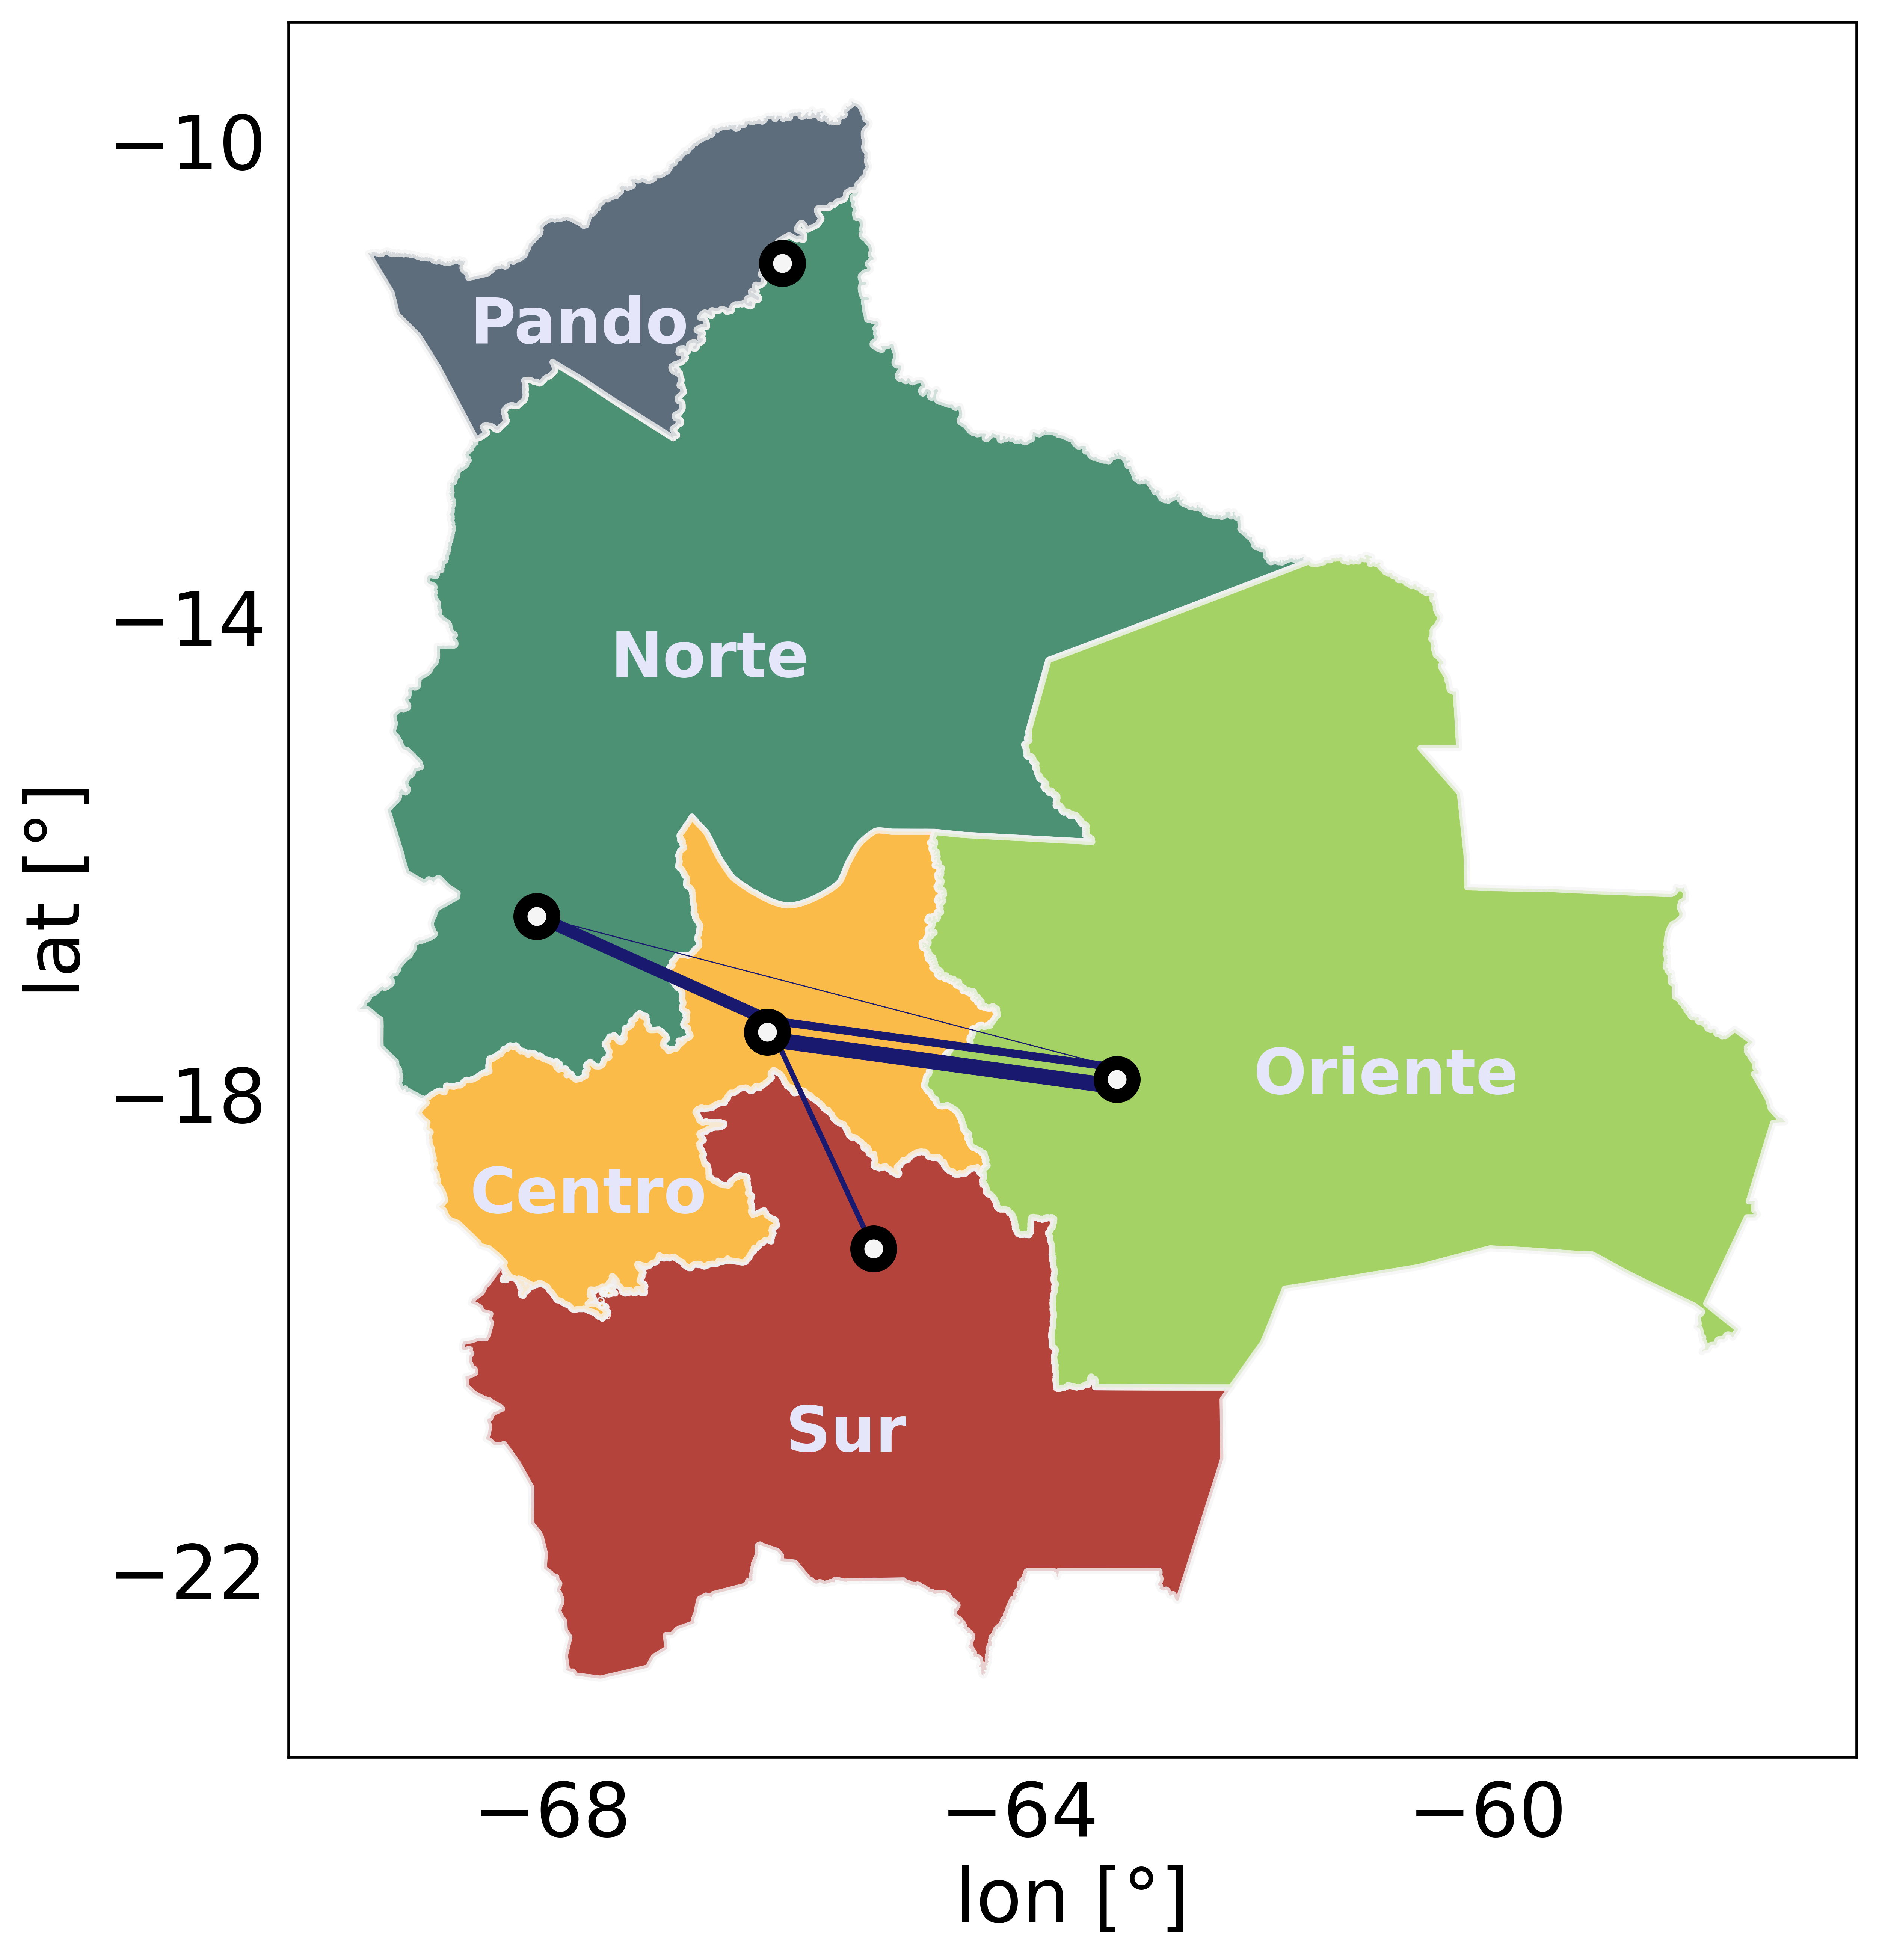
\includegraphics[clip,width=1\columnwidth]{mapas.png}
	\caption{\label{mapa} Regional nodes included in the model and power lines}
\end{figure}

\begin{table}[hb]
	\caption{Power lines}
	\label{lineas}
	\begin{tabular}{lcc}
		\toprule
		\textbf{Line} & \textbf{Nodes} & \textbf{Capacity [MW]} \\
		\midrule
		L1 & Centro-Norte & 390 \\
		L2 & Centro-Sur & 260 \\
		L3 & Centro-Oriente & 165 \\
		L4 & Oriente-Norte & 35 \\
		L5 & Centro-Oriente & 500 \\
		\bottomrule
	\end{tabular}
\end{table}

\subsection{Modeling approach}

In this study, the Low Emissions Analysis Platform (LEAP) and the Next Energy Modeling System for Optimization (NEMO) were used to model Bolivia's energy sector. LEAP is a modeling tool developed by the Stockholm Environment Institute \cite{Heaps2022LEAP}. It has been widely used by researchers and organizations to project future energy demand and supply and greenhouse gas (GHG) emissions, and to assess energy policies and scenarios \cite{emodi2017energy, shahid2021leap, handayani2023integrating}. It supports the implementation of multiple modeling approaches within a single model, including bottom-up \cite{fleiter2011barriers} and top-down methodologies \cite{rogan2014leaps}, and it allows the formulation and comparison of different energy scenarios. NEMO is an open-source tool for energy system optimization \cite{SEI2026NEMO}. Combined with LEAP, it enables additional modeling capabilities, such as least-cost optimization of energy supply and demand, multi-regional trade simulation, nodal network configuration, and energy storage modeling. In this study, we implemented a bottom-up approach and enabled NEMO's optimization module, together with the Cbc solver, for non-renewable capacity expansion, nodal simulation, and electricity dispatch.

The structure of both energy demand and supply — including regional features — was replicated in LEAP using information from national energy balances and inventories \cite{MHE2023BED, MHE2024BEN, AETN2026}, which provide annual energy demand volumes disaggregated by sector (industry, residential, transport, etc.) and by energy source (electricity, gasoline, diesel, etc.), as well as an updated generation fleet inventory. The base year of the simulation was set to 2023, and the simulation covers the 2023–2050 period.

Both power load curves as well as maximum availability curves for hydroelectric, solar and wind plants were configured with two-hourly resolution grouped in a wet season (november to april) and a dry season (may to october), resulting in 24 time slices.


\subsection{Demand}

As mentioned before, energy demand was modeled for 5 geographical regions (Pando, Norte, Centro, Oriente, Sur) and for 7 sectors: residential, transport, industry, commercial + public, agriculture + fishery + mining, and construction. For the residential sector, the number of households represents the unit of consumption. We used population projections from the national bureau of statistics (INE in Spanish \cite{INE2024CPV}) to calculate the projected number of households. Households were then disaggregated into urban and rural subsectors, and rural households were further divided into electrified and non-electrified. Final energy uses — such as cooking, water heating, food conservation, and lighting — were then characterized in terms of coverage, efficiency, fuel share, and energy intensity based on field surveys in the context of the \textit{GENERIS} project (https://generis.com.bo/). Miscellaneous thermal and electrical uses were also characterized. All electrical appliances were associated with a load curve.

The transport sector was sub-divided into: road (light-duty, medium-duty, and heavy-duty), rail, air, waterway, and cable car. The vehicle fleet was regionalized according to inventories provided by INE.

The industrial sector was disaggregated into large-scale and small-scale units \cite{sarmiento2025energia}. For small-scale units, previous sectoral surveys allowed further disaggregation into seven categories: food, beverages and tobacco; non-metallic minerals; paper, wood and furniture; machinery and metals; textiles; clothing and leather; and chemicals, plastics and pharmaceuticals. Large-scale units were classified into seven categories according to a previous sectoral survey from INE: food and beverage; cement; bricks; metals; paper, cardboard and wood; chemicals and petrochemicals; and construction materials. For this disaggregation level, we included the consumption share of different fuel types for the years 2021–2023. The fuels considered are electricity, diesel, gasoline, jet fuel, biomass, NG, and liquefied petroleum gas (LPG).

Only one energy demand growth scenario was considered in this modeling exercise. For the transport; industry; commercial and public; agriculture, fishery and mining; and construction sectors, gross domestic product (GDP) was taken as the driver of energy demand. Sub-national reports from INE allowed the regional and sectoral disaggregation of GDP. An annual growth rate of 2.8\%, based on historical trends, was considered for the simulation period. For the residential sector, the number of households was taken as the driver of energy demand. INE projects an overall population growth of 20\%, reaching a total of 13.4 MM inhabitants by 2050. Data from the last census allowed the regional and urban/rural disaggregation of population. For each region, both total population and number of households were extrapolated from the base year onward, assuming that the regional proportion remains constant — an assumption that held for the 2012–2024 period. In order to project the regional urban/rural share of households, the ratio of urban-to-rural growth rates was computed. Then, an objective function was included in the projection so that the overall projected national number of urban households matched INE's projection. 

An analysis of the current energy demand structure shows that electricity represents approximately 11.8\% of the overall energy demand. Electricity demand within the NIS is concentrated in the Oriente region (39\%), followed by Centro, Norte (22\% each), and Sur (17\%) (Figure \ref{mapa3}, panel a). The most electricity-consuming sector is residential (37\%), followed by industry (24\%); commercial and public (23\%); agriculture, fishery and mining (11\%); construction (3\%); and transport (0.4\%).

\subsection{Power supply}

As mentioned above, Bolivia's current generation mix is predominantly thermal, with hydropower as a significant secondary source. Around 70\% of installed capacity is fossil-fueled, concentrated mainly in the Oriente, Centro, and Sur regions (Figure \ref{mapa3}b)), while hydro capacity is located in the Centro and Norte regions (Figure \ref{mapa3}c)). Wind and solar capacity, which together account for less than 1\% of installed capacity, is concentrated in the Oriente and Centro/Sur regions (Figure \ref{mapa3}d)).
Against this backdrop, this modeling exercise aims to assess the impact of expanding both centralized and distributed renewable capacity in the NIS. To this end, two centralized capacity expansion scenarios were built on top of the demand growth base scenario: Business as Usual (BAU) and Alternative (ALT). Both scenarios represent the expansion of centralized renewable capacity (wind, hydro, and solar) following the official capacity expansion schedule for the 2024-2050 period.

\begin{figure*}[tp]
	%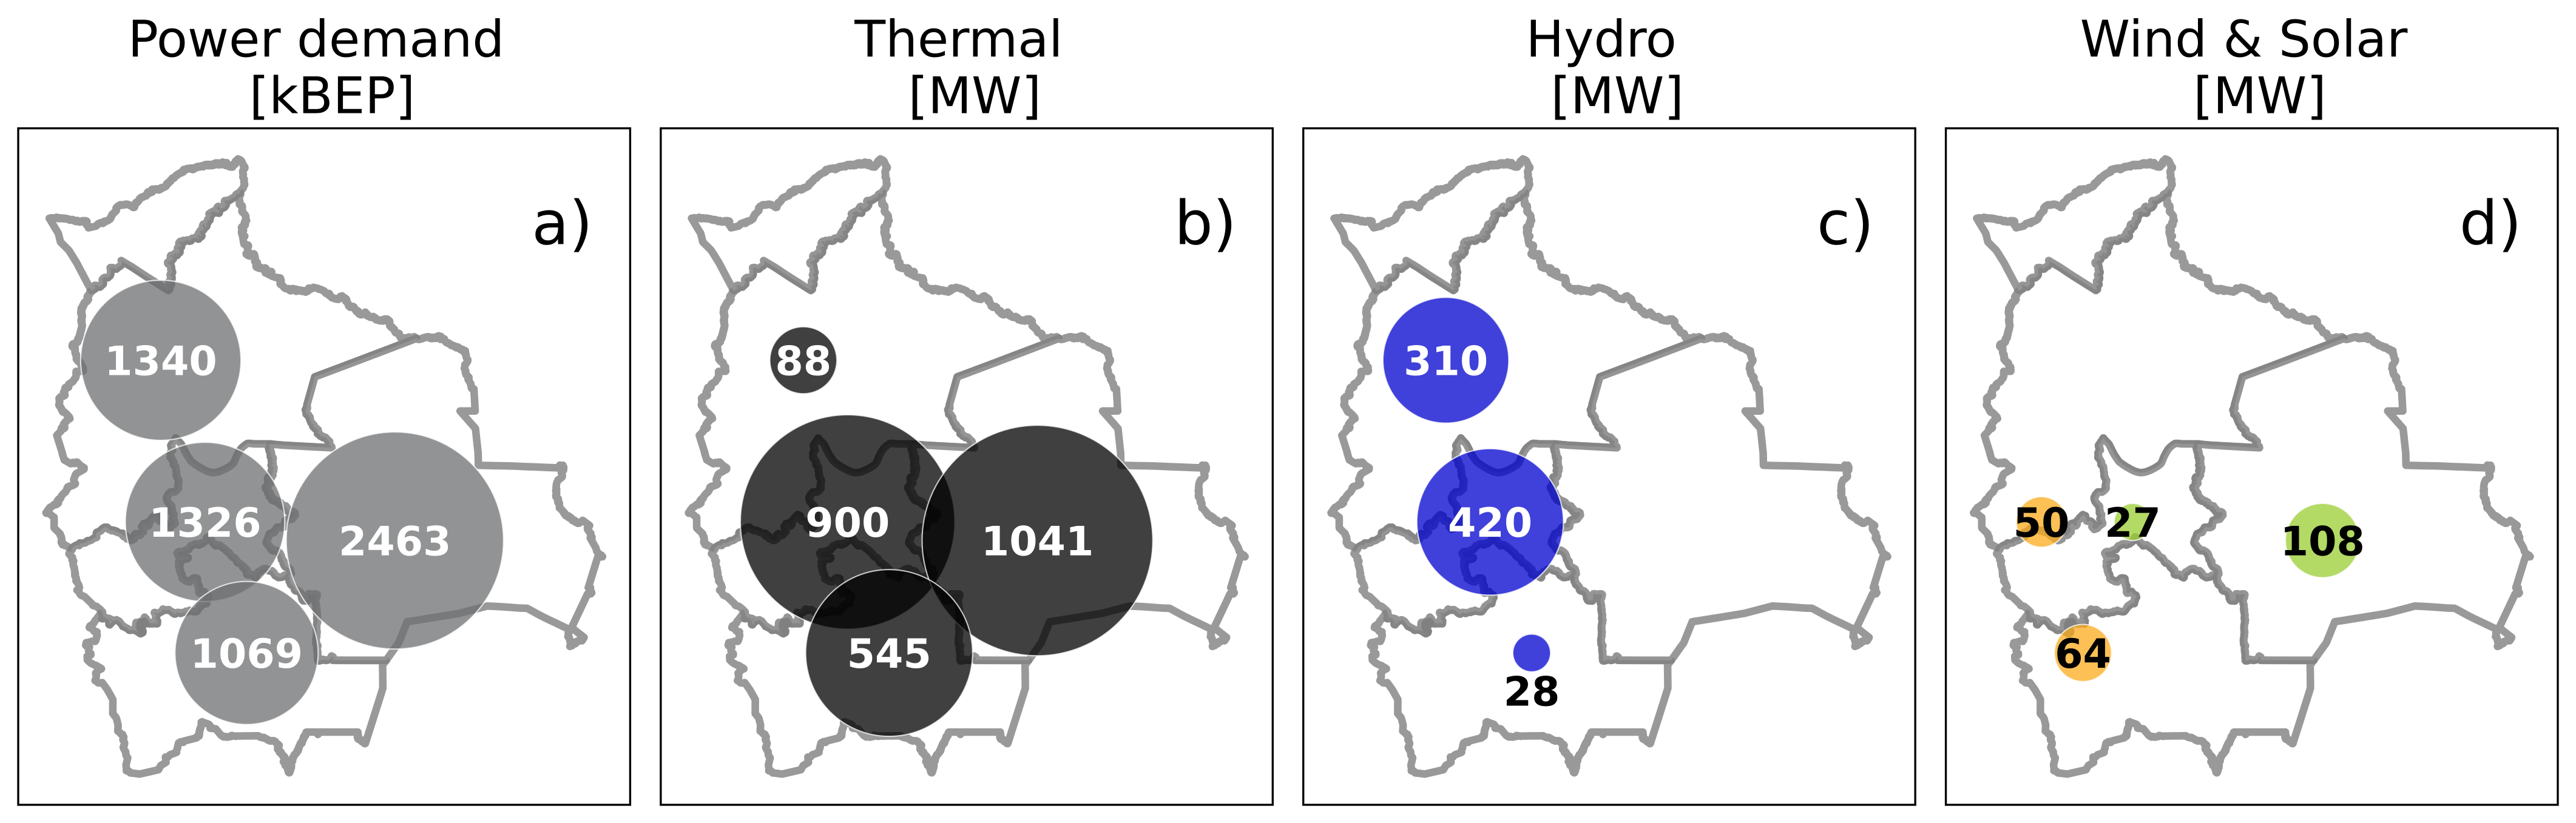
\includegraphics[clip,width=1\columnwidth]{mapas3.png}
	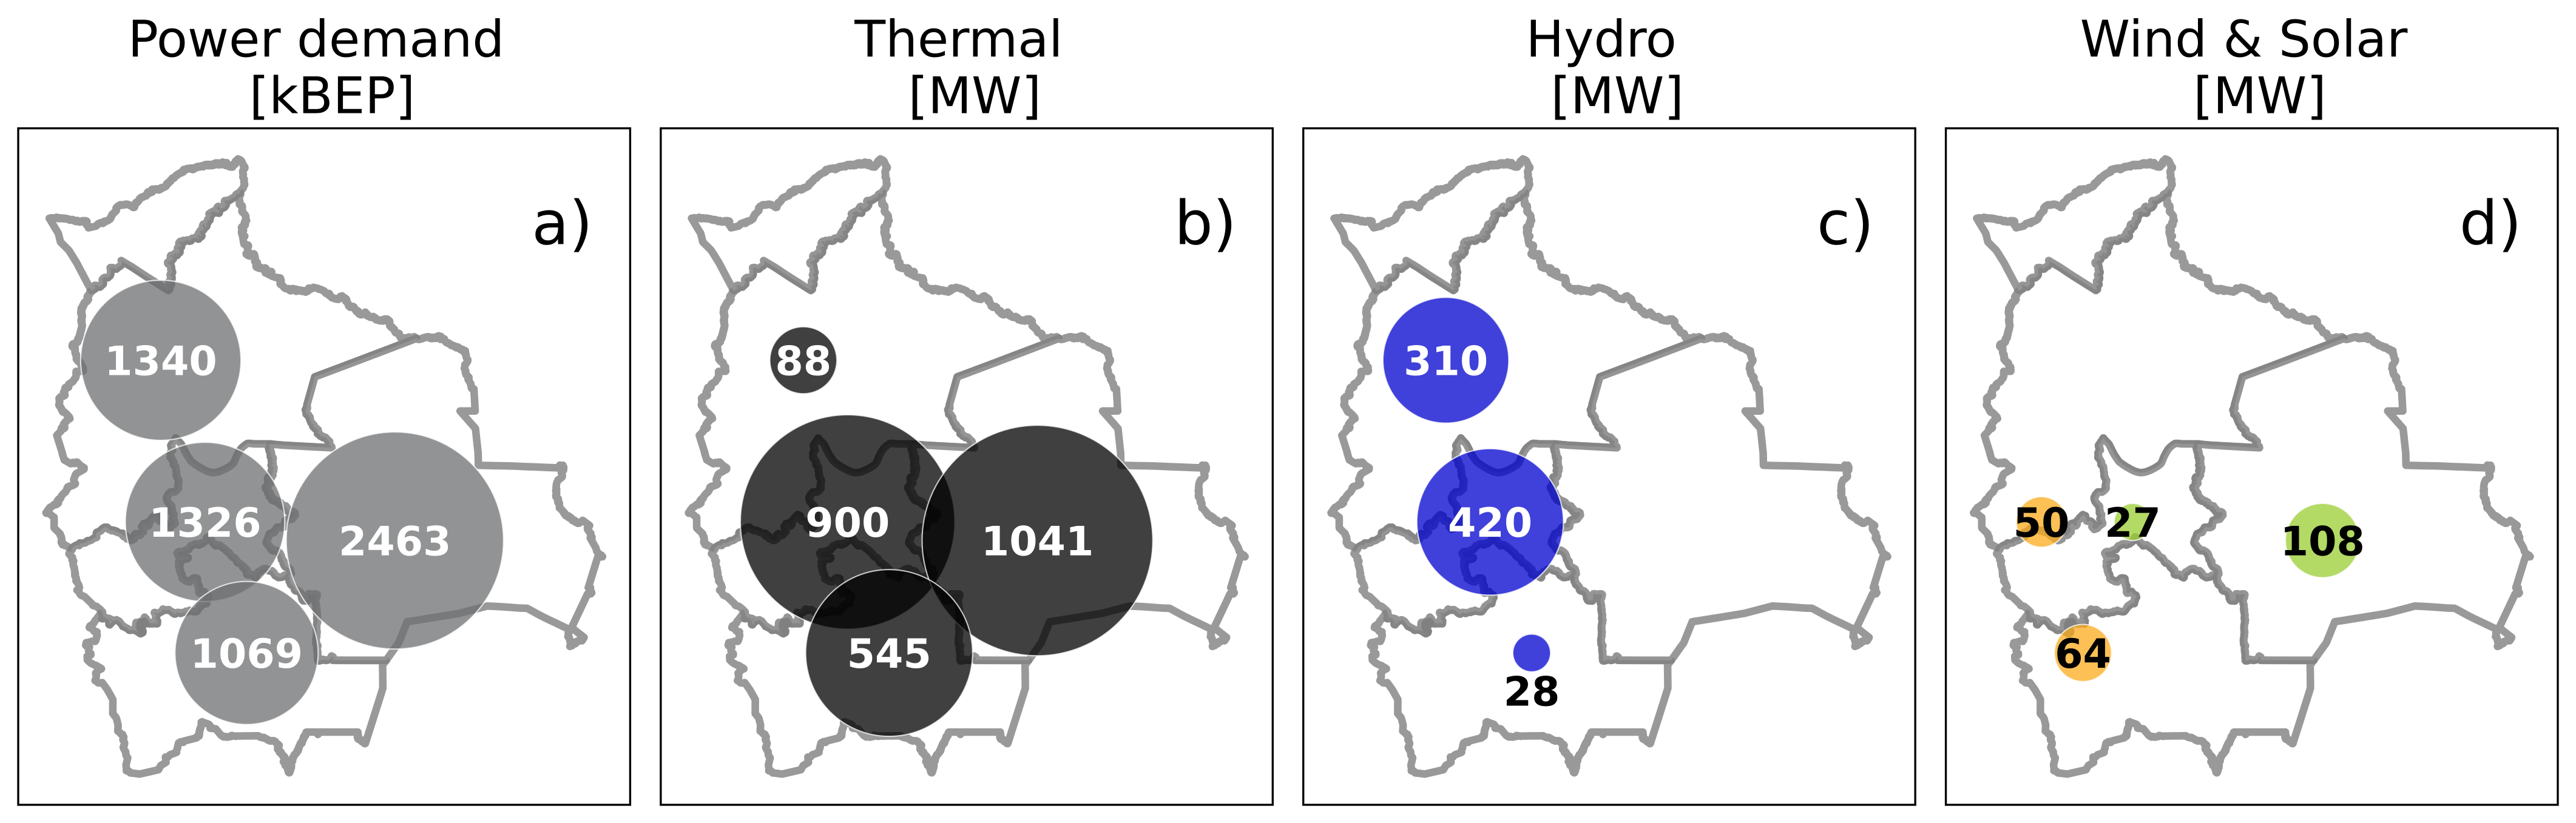
\includegraphics[width=\textwidth]{mapas3.png}
	\caption{\label{mapa3} Current annual electricity demand (a); thermal (b), hydro (c) and wind/solar (d) installed capacity}
\end{figure*}

The BAU scenario contemplates a short-term capacity expansion that includes a 261 MW addition of wind capacity in the Oriente region (Figures \ref{addition} and \ref{scenarios}). It proposes the development of two hydroelectric projects: Ivirizú (291 MW), located in the Centro region and comprising two hydroelectric plants (Sehuencas and Juntas); and Miguillas (210 MW) in the Norte region, comprising two cascade hydroelectric plants, Umapalca (91 MW) and Palillada (119 MW). It also includes the addition of 340.5 MW of solar capacity in the Centro and Norte regions. NEMO optimization assigns a total endogenous capacity of 160 MW of turbo-gas (TG) units for the simulation period for this scenario. The ALT scenario contemplates a medium-term capacity expansion that adds an additional 631 MW, 1525 MW, and 1220 MW of wind, hydro, and solar capacity relative to the BAU scenario. Wind capacity additions are concentrated in the Oriente (90\%) and Centro (10\%) regions, and are distributed in units ranging from 25 to 100 MW. Hydro capacity additions are associated with the exploitation of the Río Grande basin, and comprise the Rositas (600 MW), La Pesca (460 MW), Cañahuecal (380 MW), and Okitas (85 MW) facilities across the Centro and Oriente regions.

All centralized capacity additions were configured in LEAP as exogenous capacity additions. Maximum availability of wind, solar, and hydro was represented by availability curves derived from historical data that display intra-daily fluctuations. A minimum reserve margin of 30\% was assigned for the NIS, and differential NG production costs across regions were configured to represent the regional availability of this resource. NEMO optimization allowed for endogenous capacity expansion when needed to meet the reserve margin requirement.

\begin{figure}[hbpt]
	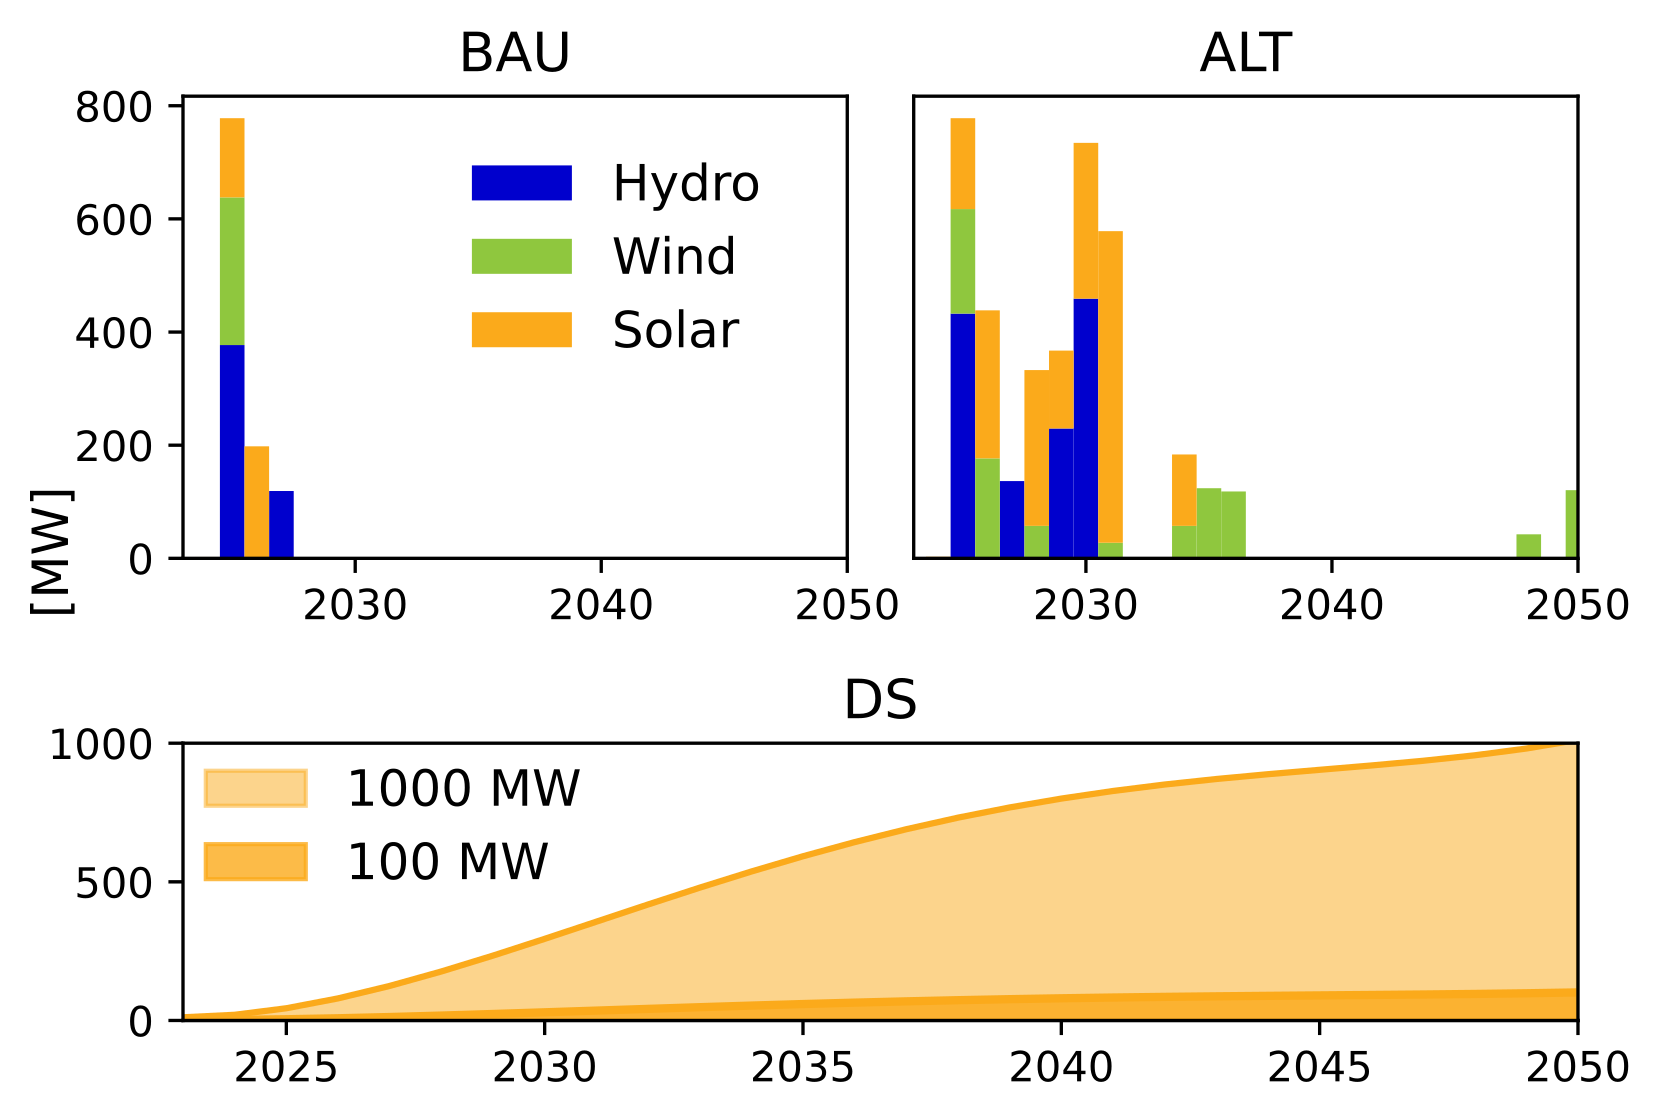
\includegraphics[clip,width=1\columnwidth]{ad.png}
	\caption{\label{addition} Centralized generation capacity additions for BAU and ALT scenarios (top row), and for DS generation (below)}
\end{figure}

Both scenarios (BAU and ALT) were then combined with two sub-scenarios representing different Distributed Solar (DS) capacity trajectories, resulting in four scenarios in total. BAU and ALT incorporate a total of 100 MW of DS capacity by 2050, whereas BAU-DS and ALT-DS incorporate a total of 1000 MW by 2050. DS capacity was added following logistic growth curves \cite{joshi2025review} (Figure \ref{addition}). DS capacity was regionally disaggregated according to current regional shares of power demand and incorporated into LEAP as a negative electricity demand source, thereby bypassing transmission and distribution losses.

\begin{figure}[hbpt]
	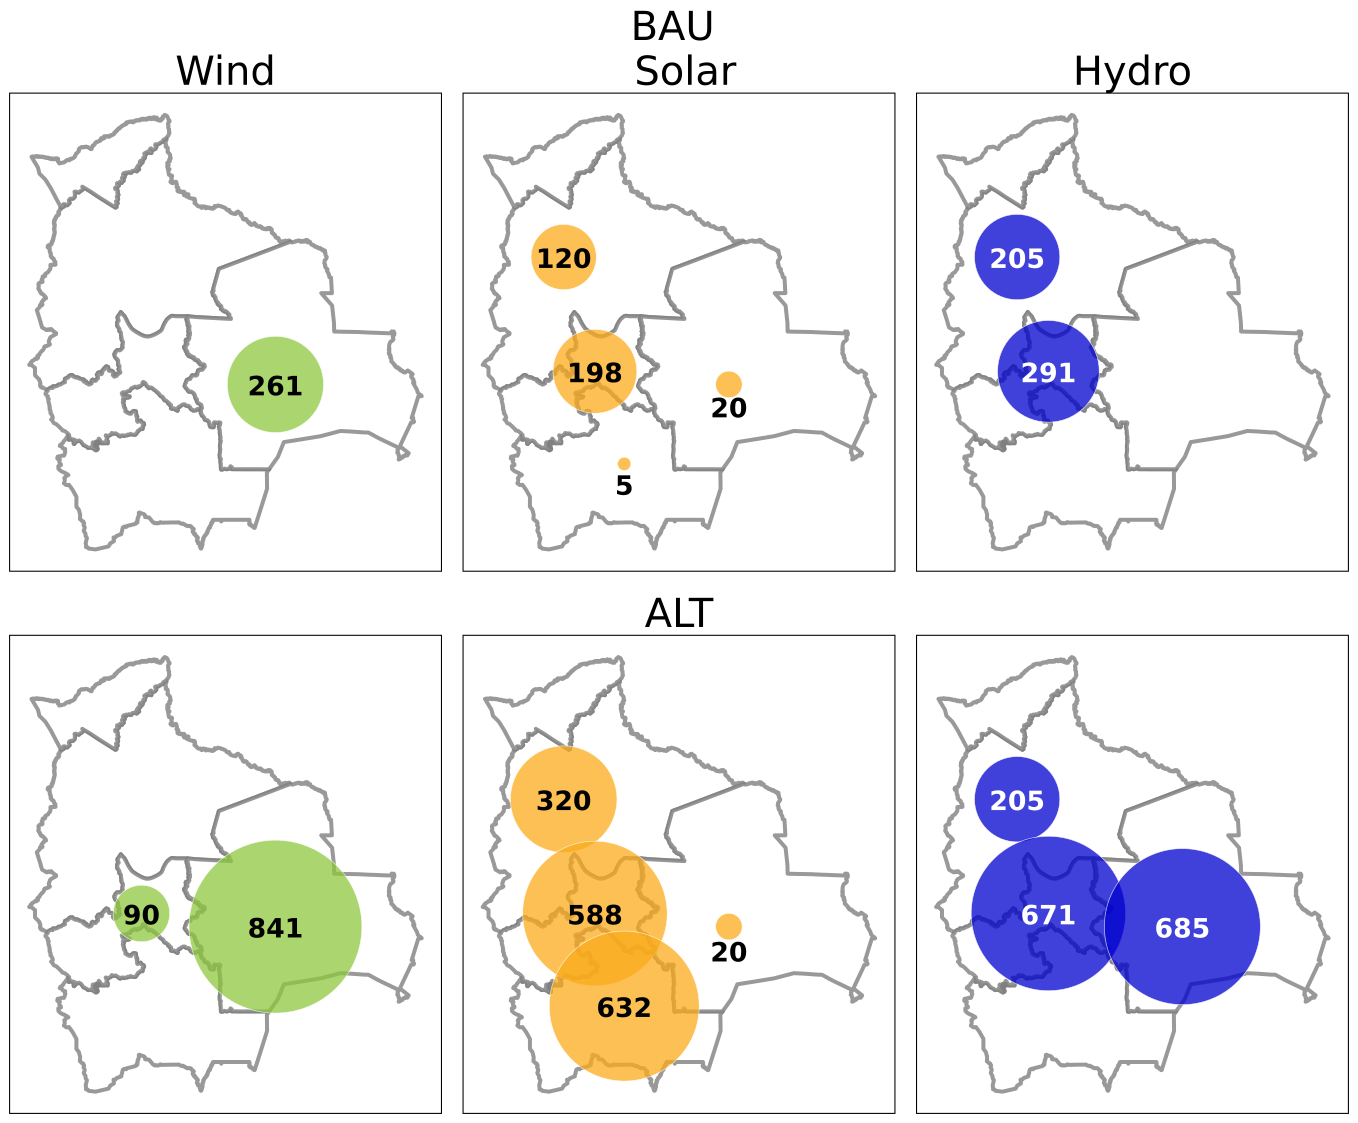
\includegraphics[clip,width=1\columnwidth]{scenarios.png}
	\caption{\label{scenarios} Regional centralized capacity additions [MW] according to BAU and ALT scenarios}
\end{figure}

For each region, we analyzed the evolution of primary and secondary energy sources within the power mix, as well as hourly power flows between regions. A regional balance of electricity generation by source and net trade was also compiled for 2050. GHG emissions were compared across scenarios using 100-year global warming potential (GWP) factors and the built-in Technology and Environmental Database, which contains emission profiles for different generation technologies from the Intergovernmental Panel on Climate Change (IPCC), the US Department of Energy, and the International Energy Agency.

Finally, a total cost analysis of the power system was performed, along with a comparison between scenarios. Total costs include capital and Operation and Maintenance (O\&M) costs for different generation technologies (see Table \ref{costos}), along with differential costs associated with displacing NG-based generation and DS installation costs. Capital and O\&M costs were incorporated into the analysis through an annual payment function that amortizes investments over time. This function accounts for equipment lifetime and the interest rate — or systemic discount rate — which was set at 12\% for the entire model. Installation and O\&M costs for new wind and solar capacity are assumed to decline over time \cite{irena2025costs}.

\begin{table}[!ht]
	\centering
	\setlength{\tabcolsep}{5pt}
	\caption{Capital and O\&M costs for different power generation technologies}
	\label{costos}
	%\resizebox{0.8\columnwidth}{!}{%
	\begin{tabular}{lcc}
		\toprule
		\text{Technology} & 	\text{Capital} & \text{O\&M} \\
	
		\textbf{} & \text{[USD/MW]} & \text{[USD/MW-yr]} \\
		\midrule
		TG & 855 & 8 \\
		TV & 1800 & 20 \\
		Diesel & 1200 & 15 \\
		CC & 1400 & 12 \\
		Solar & 1,000 & 22 \\
		Solar (new) & 850--940 & 20--22 \\
		SD & 1200 & 20--22 \\
		Wind & 1500 & 36--39 \\
		Wind (new) & 1300--1450 & 39 \\
		Hydro & 1500 & 7 \\
		Rositas (hydro) & 3350 & 38.8 \\
		Cachuela (hydro) & 1880 & 40 \\
		Río Grande (hydro) & 3446 & 39.5 \\
		Other hydro & 2029 & 29.6 \\
		\bottomrule
	\end{tabular}
\end{table}

Regarding the opportunity cost of NG — the main input for fossil-fueled generation — non-utilized NG was assumed to be available for export at a price of 5 US\$/MM BTU. A price of 120 US\$/MWh was assigned to diesel-based generation. The installation cost of DS photovoltaic panels was set at 1200 US\$/kW, comprising total capital cost and distribution adequacy costs (i.e., costs associated with reinforcing distribution infrastructure to accommodate distributed generation). Capital costs were assumed to decrease over time, while distribution adequacy costs increase, resulting in an overall installation cost that declined to 584 US\$/kW by the end of the simulation period. All values were calculated at constant 2025 prices, using the 12\% discount rate described above.

\subsection{Curtailment mitigation strategies}

An alternative balancing-oriented hydropower operation scheme has been designed and implemented in the model to manage the large volumes of renewable generation foreseen under the ALT and ALT-DS scenarios. Bolivia's current hydroelectric generation is around 2800 GWh per year, of which approximately 55\% is operated by the company ENDE Corani. A monthly analysis of the turbined-to-stored water ratio shows that only between September and November (ratios above 50\%) is there little to no margin to manage water volumes, whereas in the remaining months, around 80\% of generation could potentially be shifted to non-solar hours. The company COBEE operates around 30\% of the national hydroelectric generation. A similar analysis shows that water management is only feasible between March and June. Nevertheless, the maximum manageable energy volume was reduced from 80\% to 65\%, otherwise the maximum utilization factor would be exceeded. Up to 25\% of energy generation is available for time shifting during the dry season. Based on these analyses, an intra-daily balancing-oriented hydro operation scheme is postulated. Figure \ref{fu} a) and b) (dry and wet season respectively) shows current and proposed hydro operating schemes.

In addition to the balancing-oriented hydropower dispatch, battery storage was evaluated as an alternative for integrating renewable generation and reducing curtailment. Storage capacity was treated as an endogenous investment option, available from 2028 onwards and subject to least-cost optimization. Batteries were modeled with a [X]-hour duration, a round-trip efficiency of [Y]\%, a minimum state of charge of 15\%, and a useful life of 15 years. Under an initial capital cost of 1000 USD/kW \cite{cole2025cost}, the LEAP-NEMO optimization did not allocate any storage capacity. The capital cost was then set to zero, so that storage deployment was driven solely by system operational needs. This scenario does not represent an economically viable configuration; rather, it provides an upper bound on the curtailment reduction that storage can achieve within the modeled system and temporal resolution. Under these conditions, the model deployed up to 3100 MW of battery capacity, (reaching this level between 2037 and 2043) (Figure~\ref{fu}c).

\begin{figure*}[tp]
	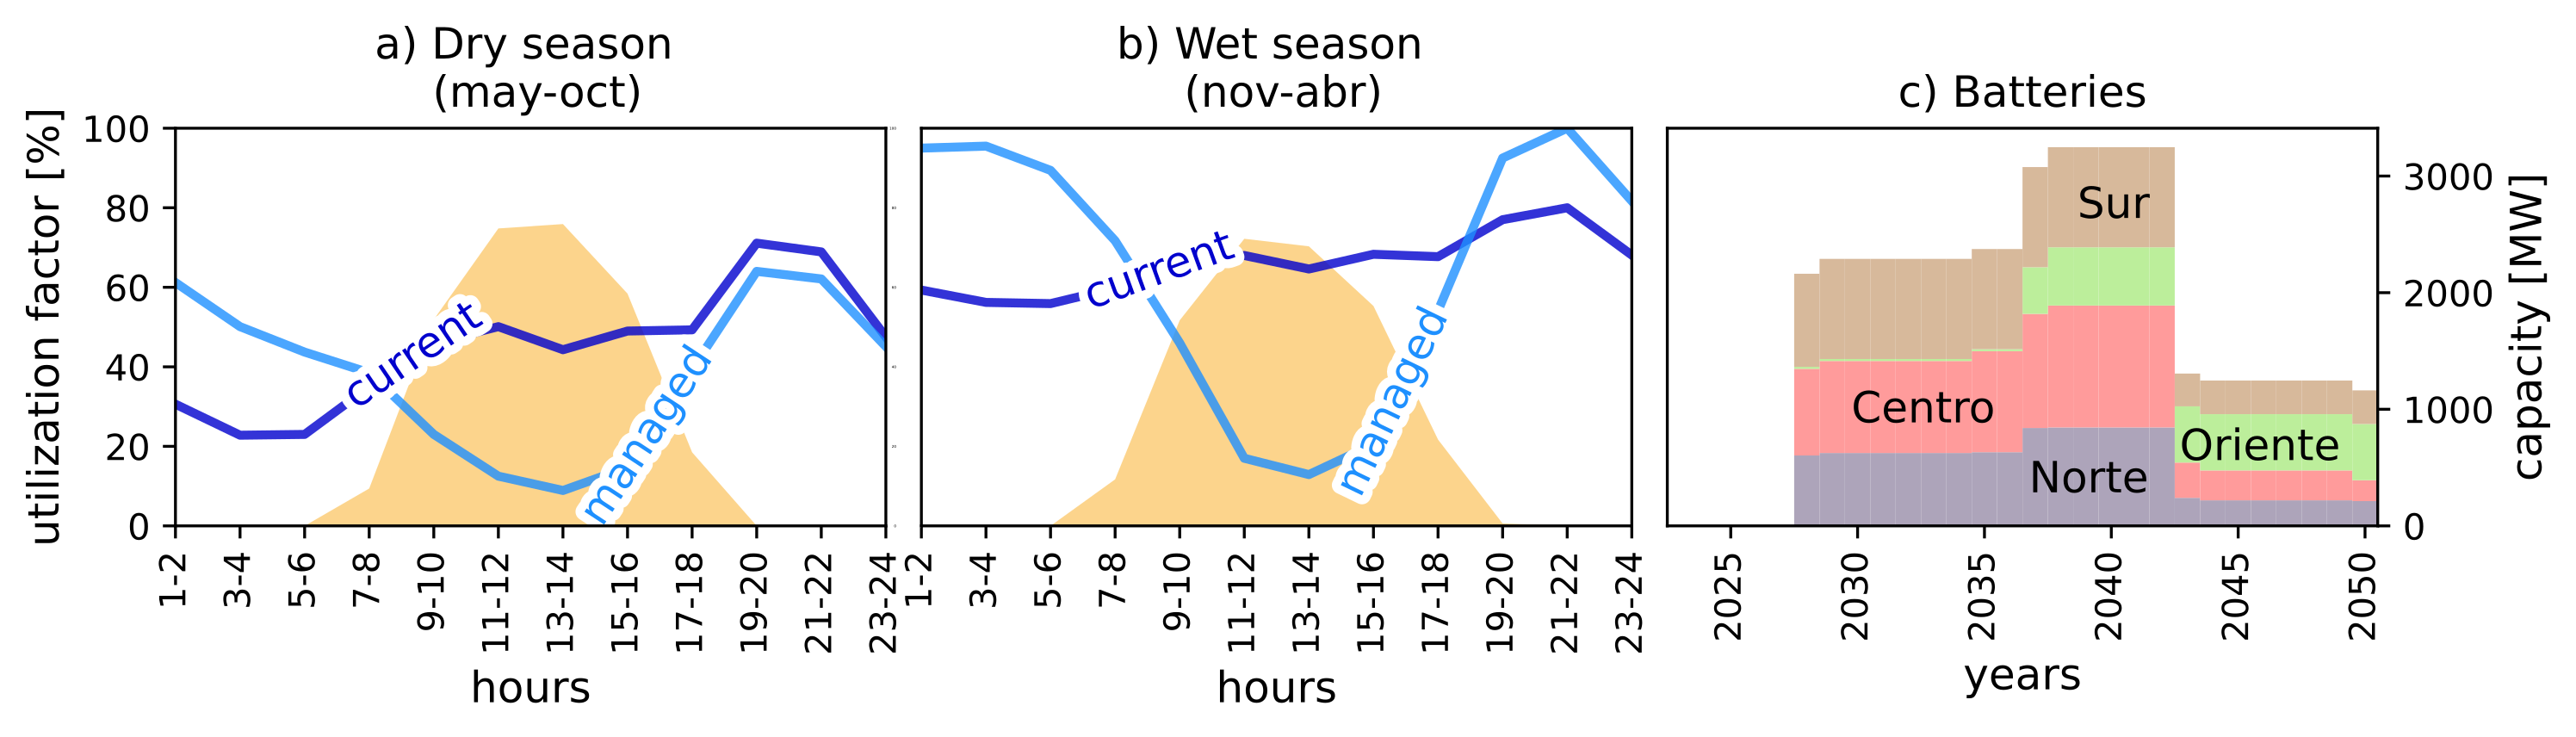
\includegraphics[width=0.9\textwidth, left]{fu.png}
	\caption{\label{fu} Current (blue line) and proposed (sky blue line) hydro hourly operation schemes and solar utilization factor (yellow area) for dry (a) and wet (b) seasons. Endogenous battery capacity additions (c)}
\end{figure*}

\section{Results}

\subsection{Demand}

The addition of DS (distributed generation) reduces the net power demand observed in the NIS. Comparison between scenarios (BAU-DS/ALT-DS vs. BAU/ALT) shows that an additional capacity of 900 MW of DS reduces net demand by about 9\% by 2050. The net accumulated energy savings over the simulation period amount to approximately 22000 and 25000 GWh, respectively, representing nearly twice the total annual demand of the base year.

\subsection{Power supply}

During the simulation period, NEMO assigned a total endogenous capacity of 160 MW of turbo-gas (TG) units under the BAU scenario, whereas no endogenous capacity expansion was observed under ALT.

Regarding power generation, the addition of DS capacity coincides with a decrease in thermal generation in both the BAU and BAU-DS scenarios. In the first scenario, DS generation represents less than 1\% of annual generation by 2050, while thermal generation escalates from 36\% in the base year to 61\% (Table \ref{generation}). In the second scenario, by contrast, DS generation represents nearly 9\% of annual generation by 2050, while thermal generation only escalates to 51\%. For the ALT and ALT-DS scenarios, there is a marked reduction in thermal generation, reaching 27\% and 26\% of annual generation by 2050, respectively, though this reduction is mostly associated with the massive deployment of centralized renewable capacity. The addition of 900 MW of DS (comparing ALT and ALT-DS) coincides with a reduction in hydro generation (42\% of annual generation in ALT vs. 37\% in ALT-DS).

\begin{table}[!ht]
	\centering
	\small
	\setlength{\tabcolsep}{5pt}
	\caption{ Current (2023) and projected (2050) annual electricity generation according to BAU, BAU-DS, ALT and ALT-DS scenarios}
	\label{generation}
	%\resizebox{0.8\columnwidth}{!}{%
		\begin{tabular}{m{1.5cm}ccccc}
			\toprule
			\textbf{} & \text{current} & \text{BAU} & \text{BAU-DS} & \text{ALT} & \text{ALT-DS} \\
			\midrule
		    Generation (GWh) & 11430 & 22410 & 20610 & 22256 & 22122 \\
			Fossil (\%) & 35.6 & 61.7 & 50.6 & 27.2 & 25.5 \\
			Solar (\%) & 0.1  & 4.3 & 4.7 & 14.8 & 14.9 \\
			DS (\%) & 0 & 0.8  & 8.6 & 0.8 & 8 \\
			Wind (\%) & 12 & 6.1  & 6.7 & 14.4 & 14.5 \\
			Hydro (\%) & 47.1 & 27.1  & 29.5 & 42.8 & 37.1 \\
			\bottomrule
		\end{tabular}
	\end{table}


The addition of DS capacity produces positive externalities in terms of fuel savings and GHG emissions. An additional 900 MW of DS capacity produces greater fuel savings for the BAU scenario than for the ALT scenario. Fuel savings for the BAU-DS scenario reach 960 kBEP annually by 2050 compared to BAU, with accumulated savings of 15000 kBEP over the simulation period — nearly the total inputs for power generation in the base year. For the ALT-DS scenario, by contrast, accumulated savings total only 1930 kBEP compared to ALT. GHG emissions follow a similar pattern: accumulated emission savings are greater for the BAU-DS scenario compared to BAU (9.9 MM metric tonnes of CO\textsubscript{2}-equivalent) than when comparing the ALT-DS scenario with ALT (1.17 MM metric tonnes of CO\textsubscript{2}-equivalent).

Overall costs related to the NIS present differences across scenarios. Costs are higher for the ALT scenario ($\approx$3600 MM USD) than for the BAU scenario. Fuel-related savings of around 1000 MM USD are exceeded by higher capital costs (see Table \ref{costostot}). The addition of DS capacity produces modest increases in overall costs: 185 and 206 MM USD for BAU-DS and ALT-DS compared with BAU and ALT, respectively. Savings related to fuel replacement are higher for BAU-DS, since DS generation replaces thermal generation. In ALT-DS, by contrast, DS generation displaces a higher proportion of centralized renewable generation.

\begin{table}[!ht]
	\centering
	\setlength{\tabcolsep}{5pt}
	\caption{Costs (BAU \& ALT scenarios) and differential costs (BAU-DS \& ALT-DS scenarios). Values are expressed in MM USD}
	\label{costostot}
	%\resizebox{0.8\columnwidth}{!}{%
		\begin{tabular}{lccccc}
			\toprule
			\textbf{} & \text{BAU} & 	\text{(BAU-DS)} & \text{ALT} & \text{(ALT-DS)} \\
			\textbf{} & \text{}  & \text{-BAU} & \text{} & \text{-ALT} \\

			\midrule
			Fuel & 2227 & -171 & 1192 & -25 \\
			Capital + O\&M & 6963 & -1 & 11605 & -128 \\
			SD panels & 39  & 360 & 39 & 360 \\
			Total & 9230  & 185 & 12837 & 206 \\
		
			\bottomrule
		\end{tabular}
	\end{table}

\subsubsection{Regional power generation and trade projections}

As mentioned earlier, the regionalized model of Bolivia's energy system includes electricity exchanges between regions, for which the main transmission lines have been represented. This section presents an hourly analysis of power flows between regions for three time slices (years 2030, 2040, and 2050), together with the evolution of power generation sources over the simulation period. Simulated power flows did not exceed the maximum transmission line capacities during the simulation period. Different capacity thresholds were configured and tested in sensitivity scenarios, and results showed no differences compared to the reference scenarios.

For the BAU scenario, in the first time slice it can be observed that the Centro region — where hydroelectric generation predominates (first row in Figure \ref{inputBAU}) — is the main electricity exporter (first and third rows in Figure \ref{tradeB}), followed by the Oriente region. Exports are directed toward the Sur region, Norte region —during dry-season early morning hours—, and Oriente region —during midday and afternoon periods—. In all three importer regions, generation is predominantly thermal.

The second time slice, 2040, shows similar daily export features, and the Sur region adds exports during nighttime and morning hours. Norte region imports energy throughout the day, and imports are greatly diminished in the Oriente and Sur regions compared to the first time slice. This displacement of Sur/Oriente by Norte as the main importers of energy responds to the fact that NEMO augments thermal-based generation in the Sur and Oriente regions due to greater availability of NG and thermal generation capacity in these regions, while overall capacity remains nearly unchanged in the Norte region. In this way, the Centro region acts as a transit node between Sur and Norte. 

For 2050, almost all exports are made from the Centro region, while imports are directed mainly to Norte, followed by Oriente. Overall generation barely increases for this time slice in Norte. The observed increase in thermal generation in Oriente (from approximately 10000 GWh to 15000 GWh) does not appear sufficient to meet regional demand, which is instead covered by imports from Centro.

\begin{figure*}[tp]
	%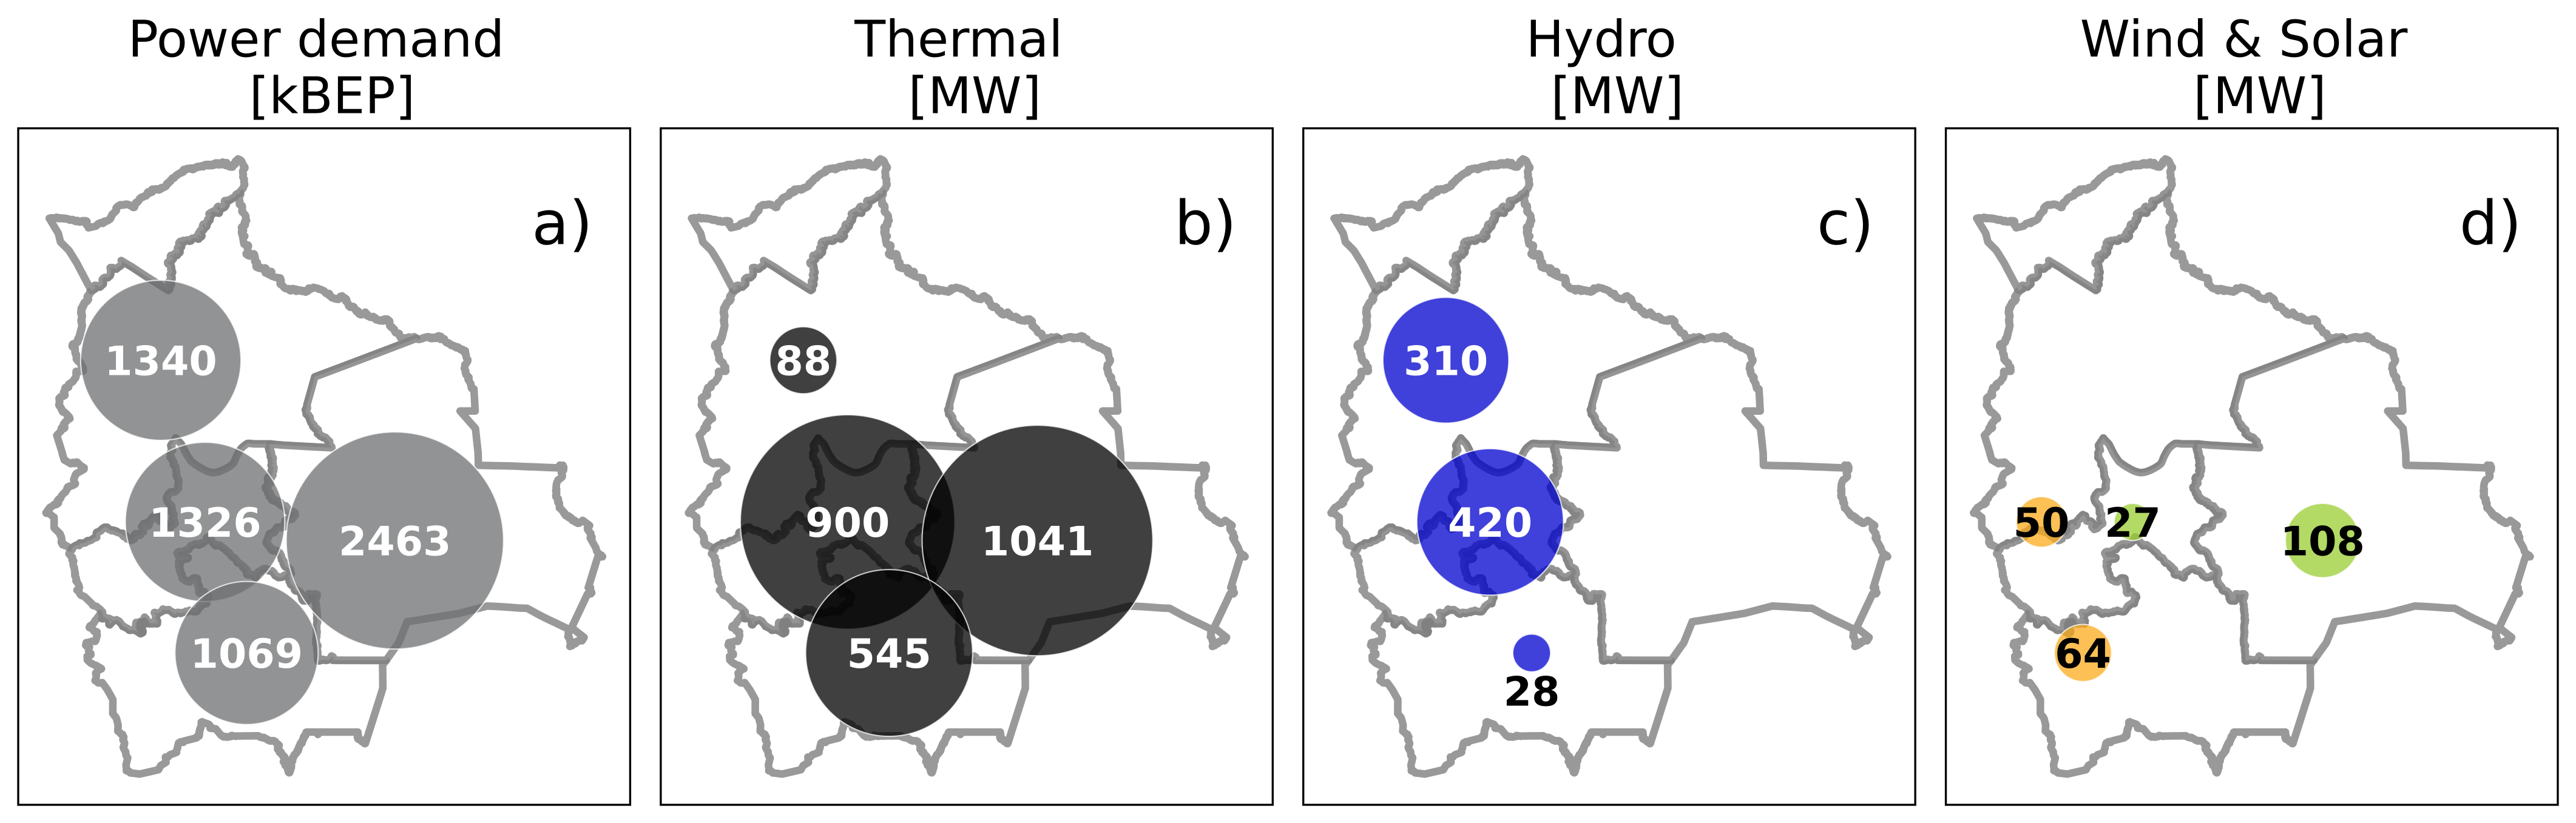
\includegraphics[clip,width=1\columnwidth]{mapas3.png}
	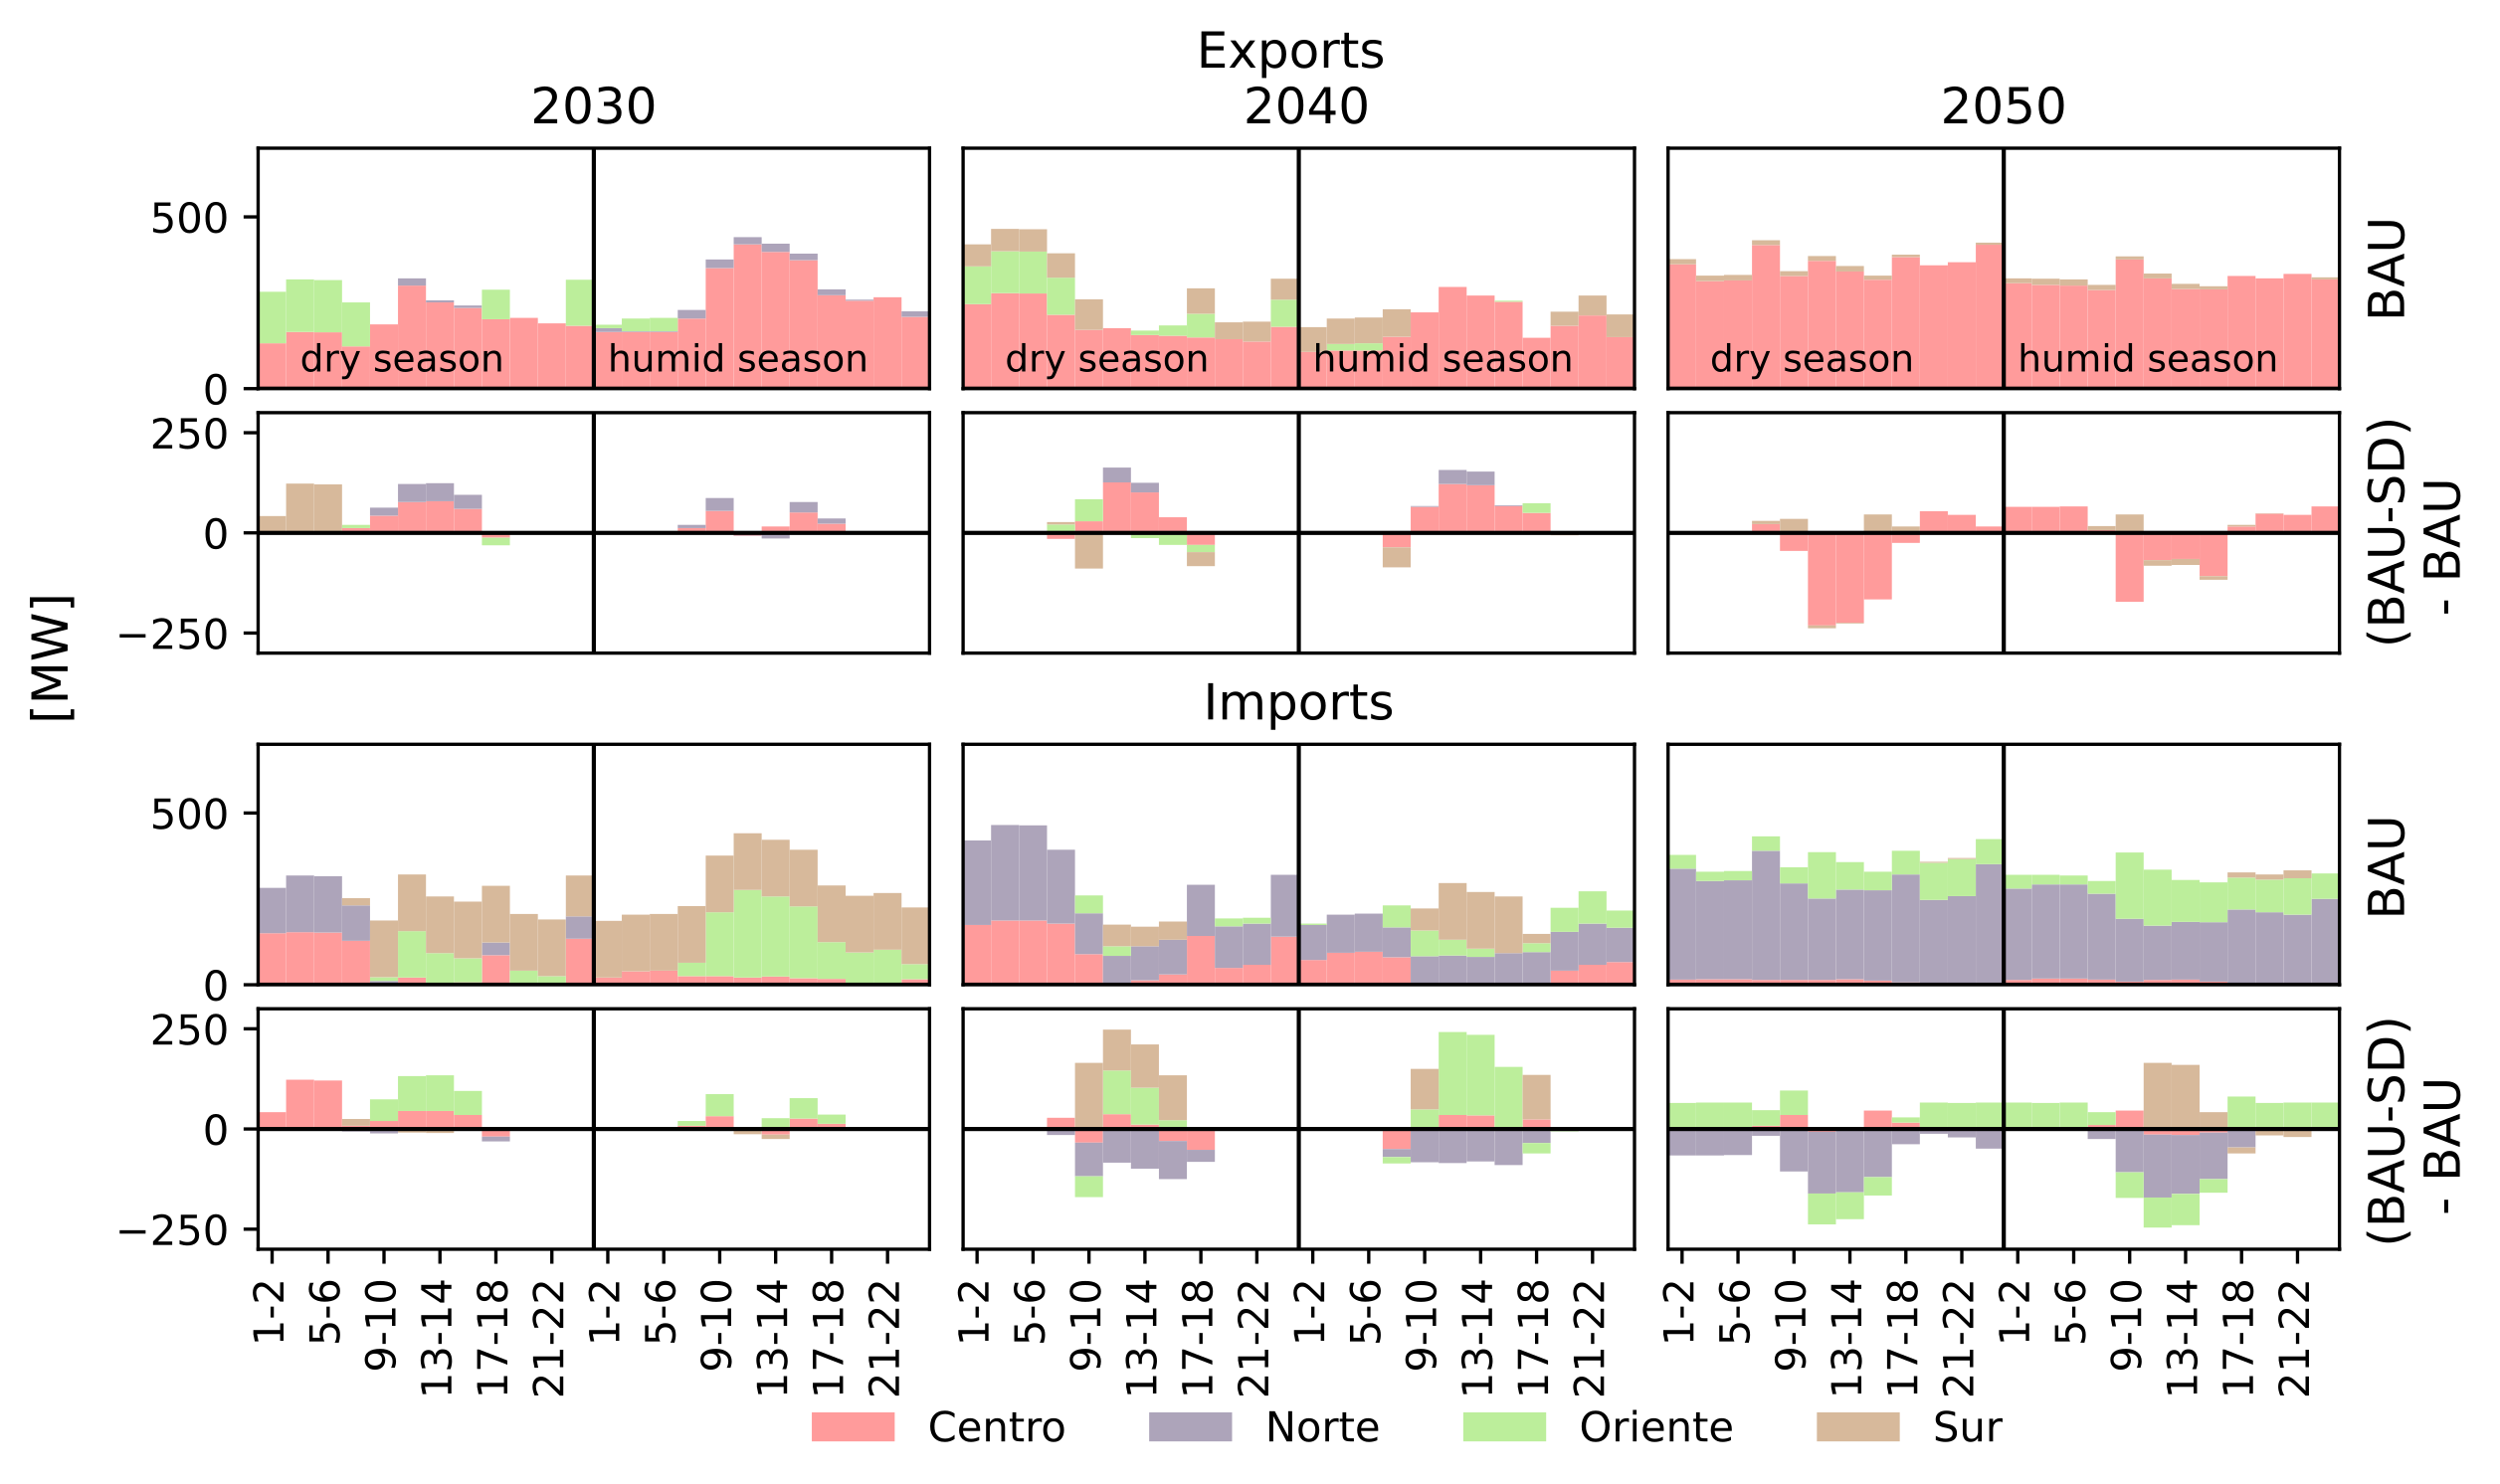
\includegraphics[width=\textwidth]{tradeTEN.png}
	\caption{\label{tradeB} Daily profiles of inter-regional exports and imports of power flow for BAU scenario (first and third row), and differences for BAU-DS scenario (second and fourth row)}
\end{figure*}

An additional 900 MW of DS capacity (BAU-DS scenario) translates into modifications in both daily exports/imports and generation features across regions. For 2030, there are marginal increases in exports during solar generation hours from the Norte region, whose generation is predominantly renewable (second and fourth rows in Figure \ref{tradeB}, and lower row in Figure \ref{inputBAU}). There is also an increase in imports directed to Oriente, which coincides with a local decrease in thermal generation. 

For 2040, the addition of extra DS capacity produces an increase in exports from the Centro region . Imports are diminished in the Norte region, while increasing in Oriente and Sur, whose annual thermal generation is in turn reduced by approximately 1500 and 1000 GWh, respectively.

Finally, for the year 2050, the BAU-DS scenario foresees diminished thermal generation in the Centro, Oriente, and Sur regions. Besides, imports during solar generation hours are diminished in the Norte and Oriente regions. These decreases in imports to Norte and Oriente are, in part, compensated by an increase in imports from Sur, whose generation share is entirely thermal.

\begin{figure*}[tp]
	%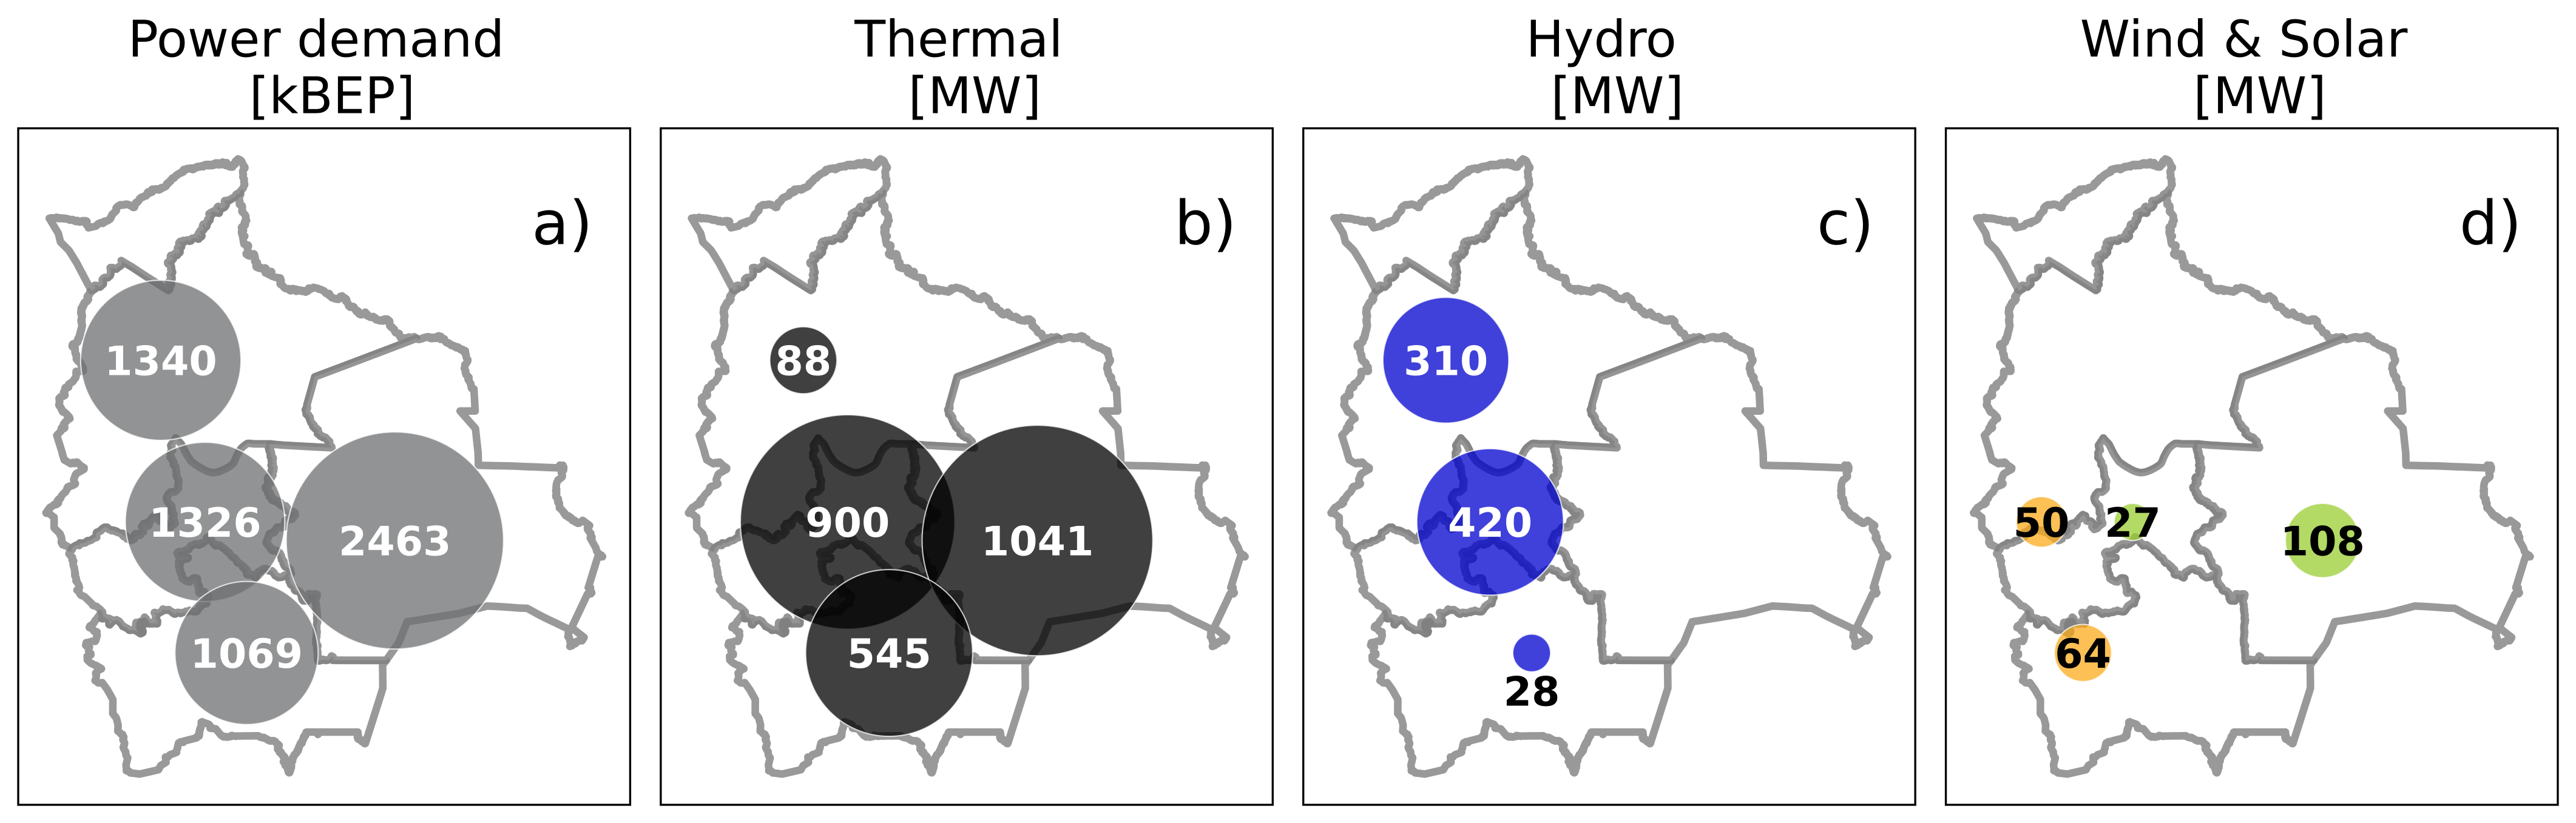
\includegraphics[clip,width=1\columnwidth]{mapas3.png}
	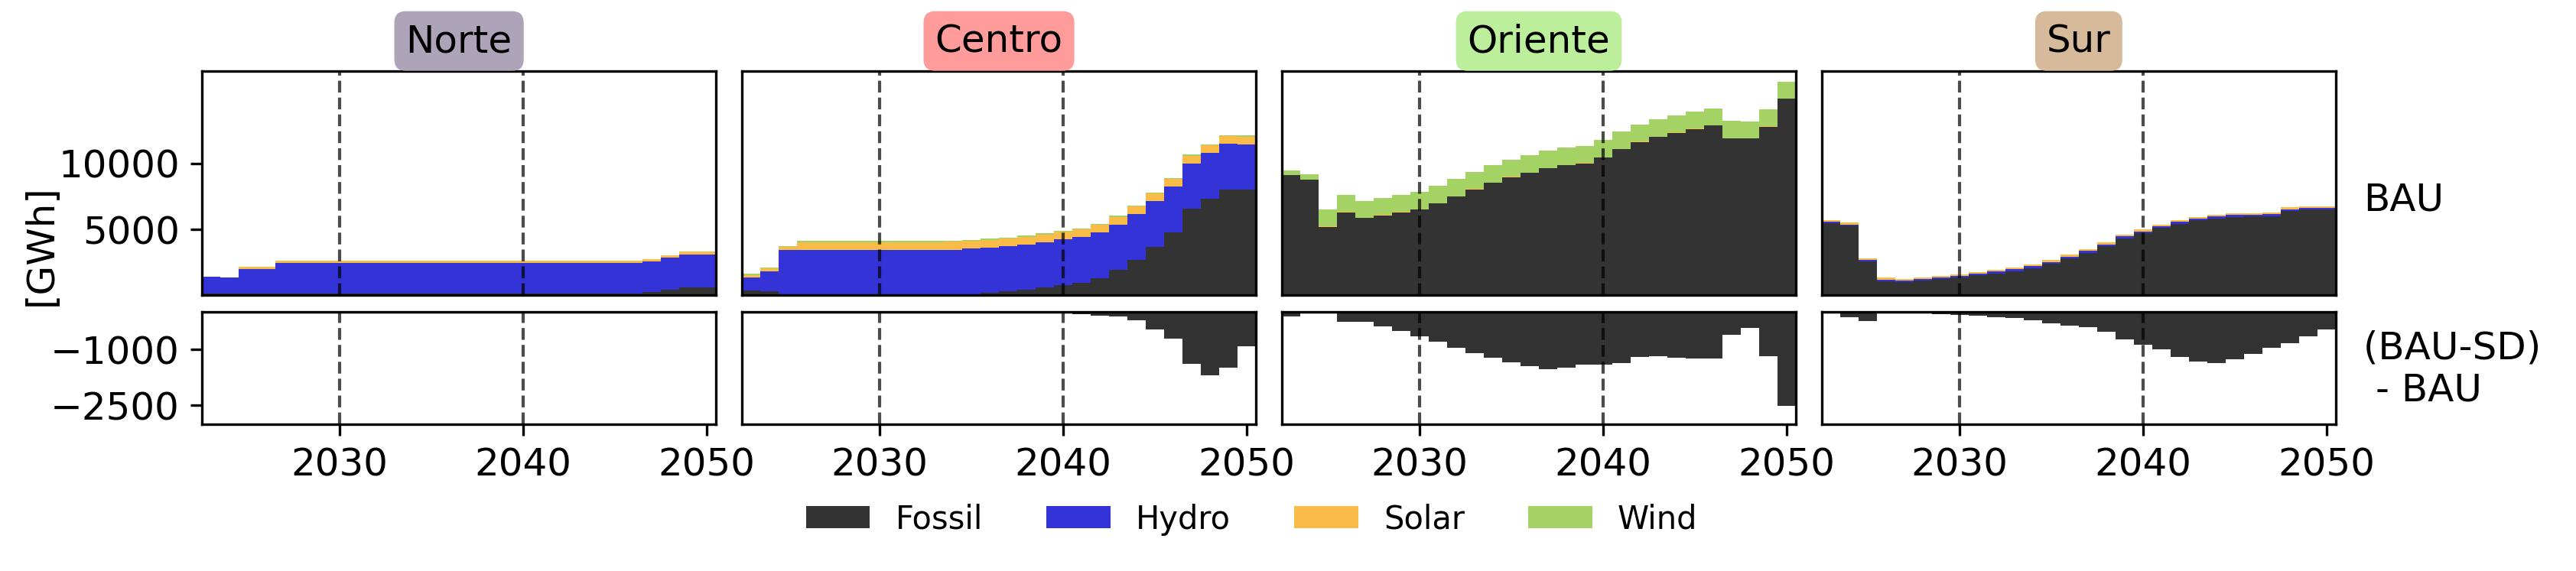
\includegraphics[width=\textwidth]{inputTEN.jpg}
	\caption{\label{inputBAU} Evolution of regional projected annual electricity generation according to BAU scenario (upper row), and differences for BAU-DS scenario (lower row)}
\end{figure*}

For the ALT scenario, inter-regional power flows vary across seasons and time of day. For the year 2030, Oriente is the main electricity exporter during the dry season (top row in Figure \ref{tradeA}), sending power to Norte. Sur region switched from exporter during the first part of the day to importer during the evening. During the wet season, energy flows from Oriente and Centro toward Sur region, except during solar production hours, when the high share of solar generation in Sur (top row in Figure \ref{inputALT}) produces a surplus that is instead exported toward Norte region. It is also worth noting the substantial hydro and wind generation output of Oriente region in this scenario, which underpins its role as a net exporter throughout the year.

For the year 2040 Oriente and Sur are still the main electricity exporting regions showing a similar daily scheme to 2030. Exports are directed towards the Norte region, whose overall generation barely varies since 2030 (Figure \ref{inputALT}). Imports from the Sur region during nighttime hours in the humid season cease.

Distinct interregional trade patterns emerge during non-solar and solar generation hours at the end of the simulation period. During non-solar generation hours, energy flows from Centro and Oriente towards the Norte region. During solar generation hours, Centro and Sur—whose solar generation is the greatest among the regions—export electricity to Norte and Oriente, the latter having no centralized solar generation.


\begin{figure*}[tp]
	%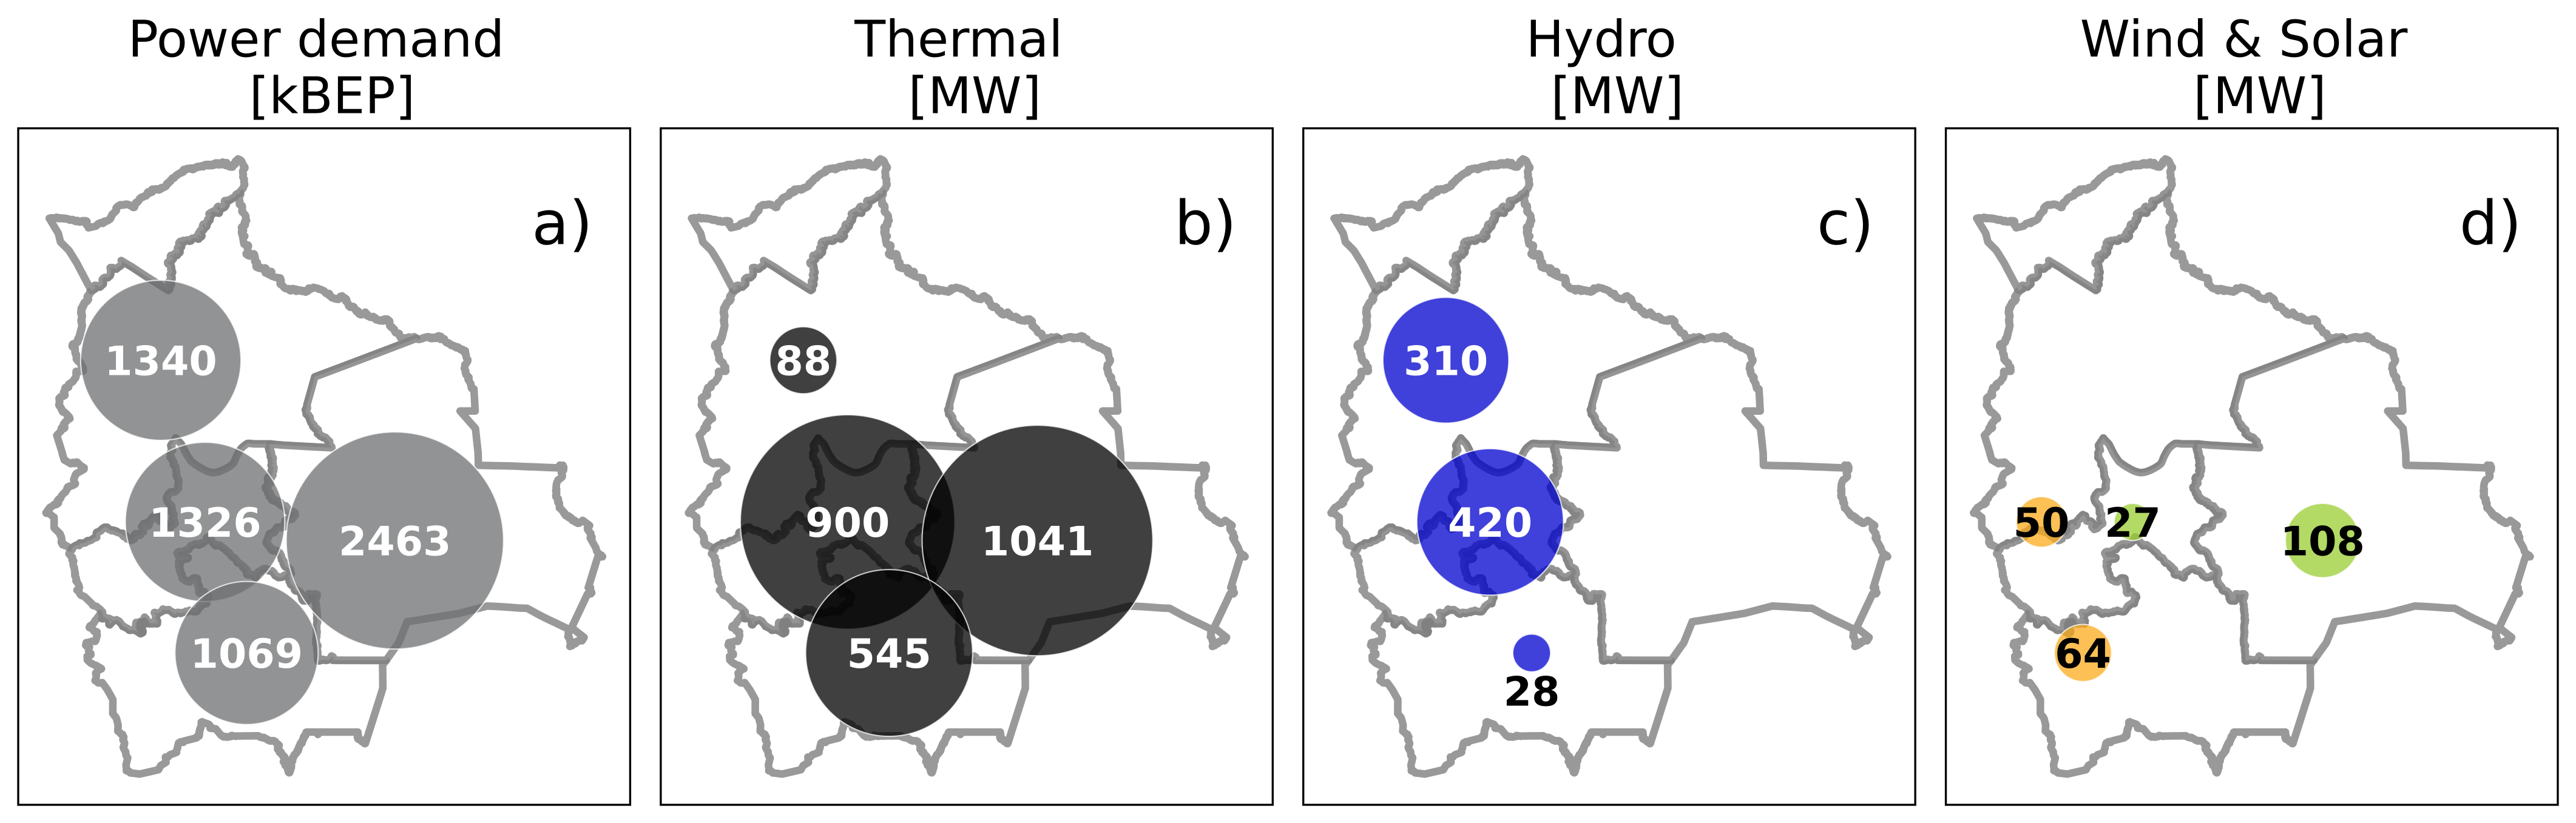
\includegraphics[clip,width=1\columnwidth]{mapas3.png}
	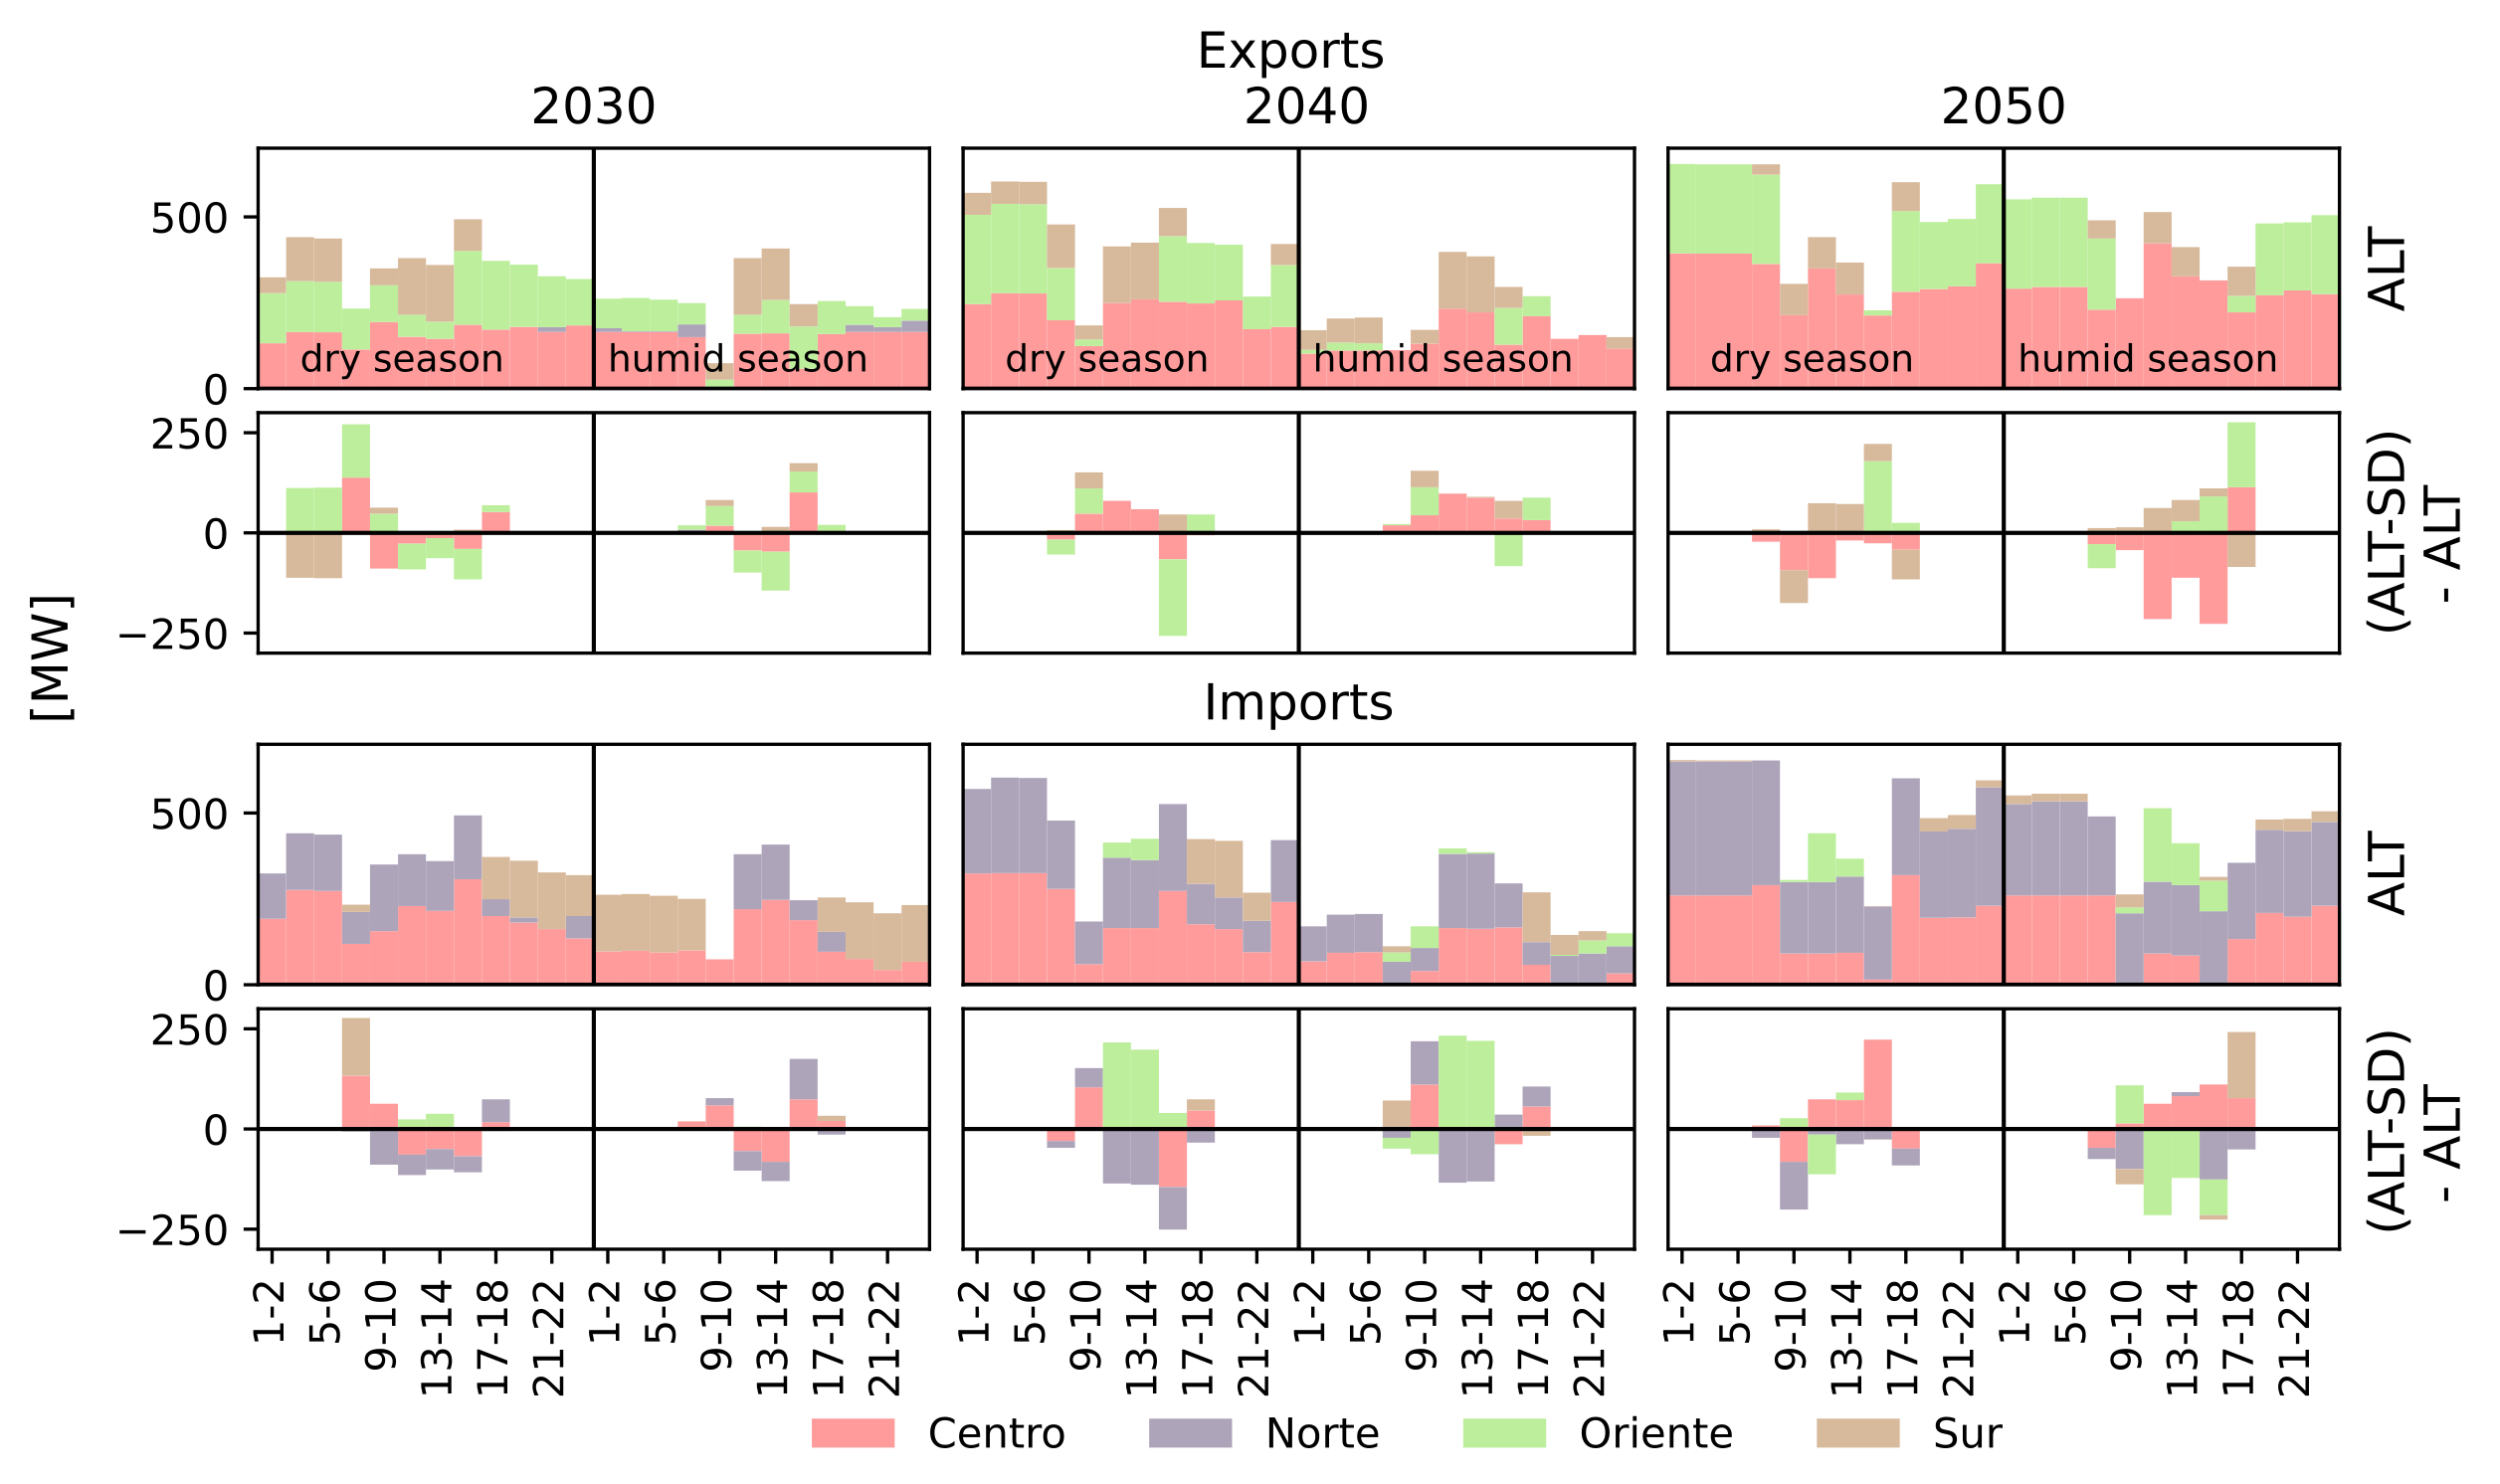
\includegraphics[width=\textwidth]{tradeALT.png}
	\caption{\label{tradeA} Daily profiles of inter-regional exports and imports of power flow for ALT scenario (first and third row), and differences for ALT-DS scenario (second and fourth row)}
\end{figure*}

The additional 900 MW of DS capacity in the ALT-DS scenario, compared to BAU-DS, leads to different effects due to the overall higher renewable installed capacity. This produces greater temporal overlap between renewable generation sources, reducing hydro output (bottom row in Figure \ref{inputALT}). For 2030, exports from Oriente and imports from Centro and Sur decrease during solar production hours. During the dry season, morning imports shift from Sur to Oriente (bottom row in Figure \ref{tradeA}). Compared to the ALT scenario, hydro generation is reduced in the Norte, Centro, and Oriente regions, while thermal generation is displaced in Sur.

During 2040, exports from the Centro region increase, while imports switch from Norte to Oriente during solar production hours. Hydro generation diminishes in the Oriente region compared to 2030. Finally, during 2050, there is an overall decrease in imports from the Oriente and Norte regions during solar production hours. Hydro generation is further reduced in the Centro region, while the Oriente and Sur regions experience a reduction in thermal generation.

\begin{figure*}[tp]
	%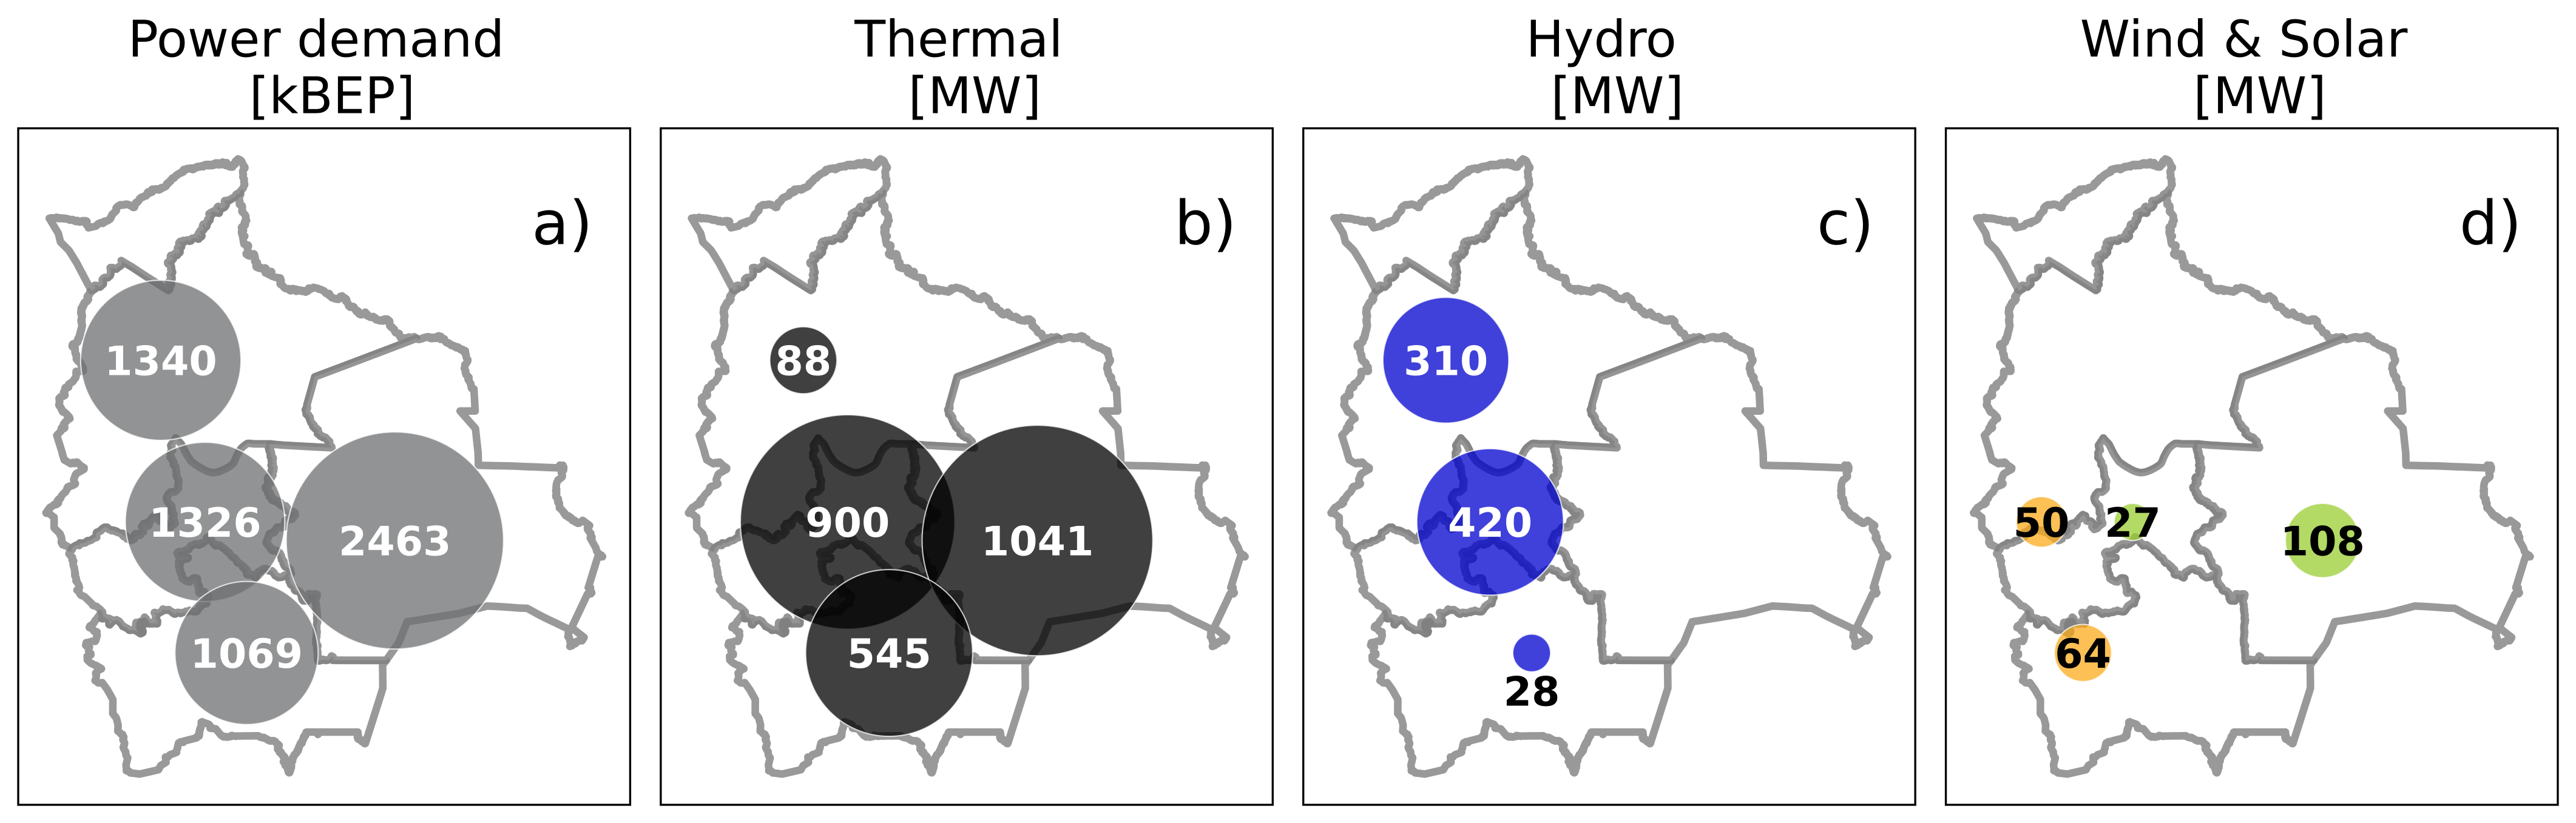
\includegraphics[clip,width=1\columnwidth]{mapas3.png}
	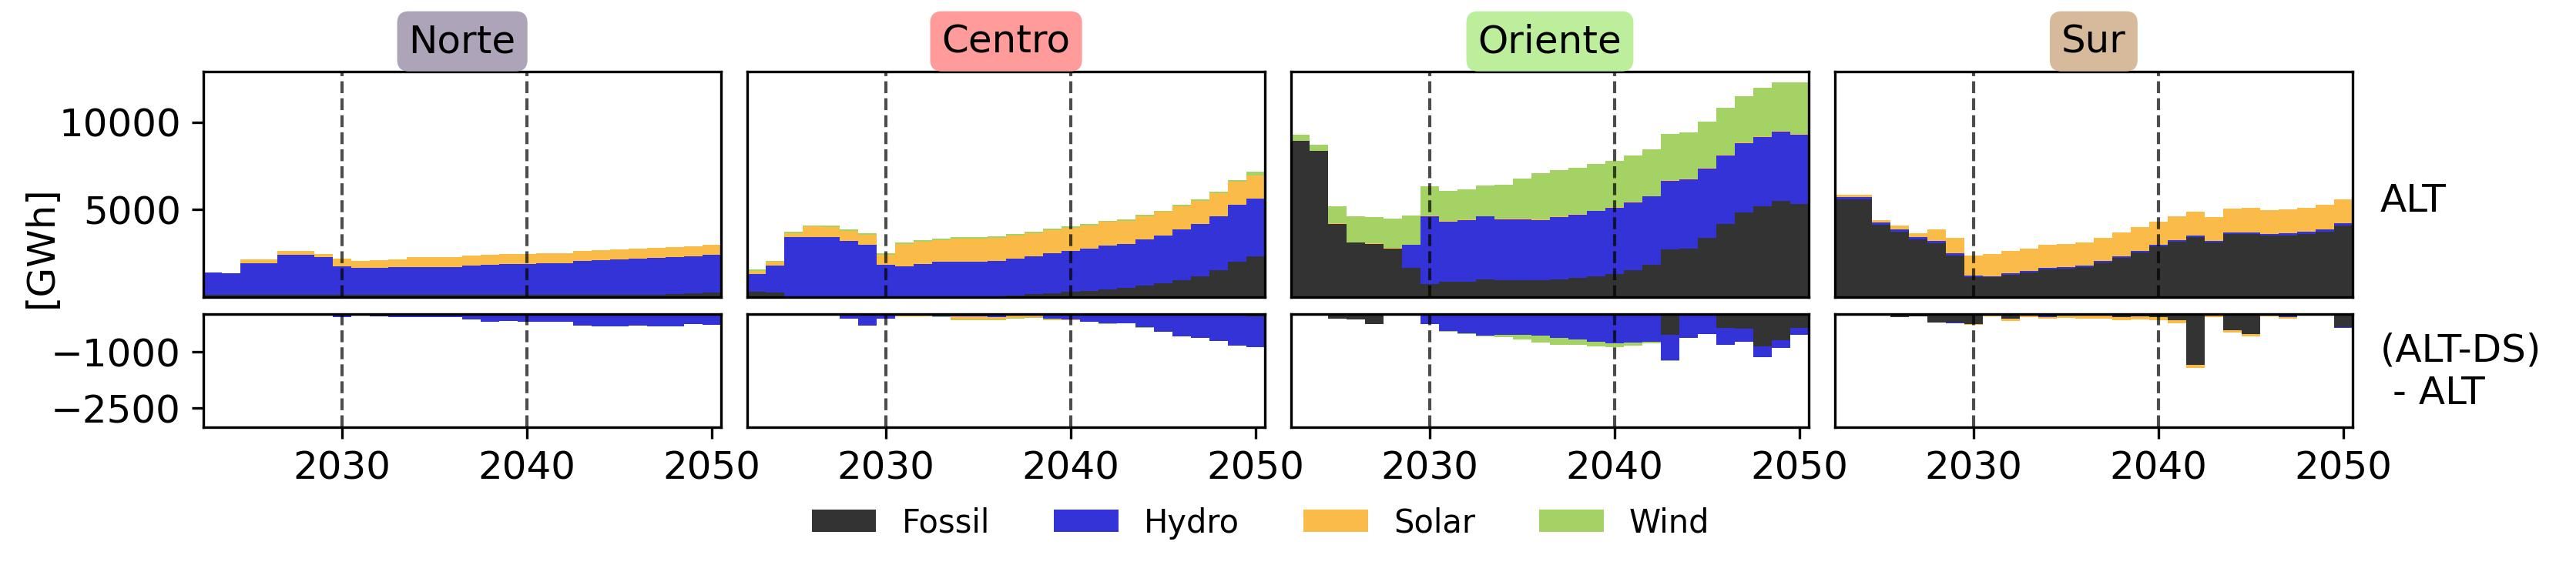
\includegraphics[width=\textwidth]{inputALT.jpg}
	\caption{\label{inputALT} Evolution of regional projected annual electricity generation according to ALT scenario (upper row), and differences for ALT-DS scenario (lower row)}
\end{figure*}


\subsection{Energy curtailment}

One of the most salient results of the simulation concerns the combined effect of DS and centralized renewable penetration in the ALT scenario. This scenario assumes higher centralized renewable capacity than BAU, and the additional DS capacity further contributes to an oversupply of renewable generation during hours of high solar output (Figure \ref{pow2}). In the BAU scenario, the addition of 900 MW of DS capacity leads to a reduction in thermal generation of approximately 760 GWh/year by 2050 (Figure \ref{inputBAU}), whereas in the ALT scenario, DS penetration instead displaces a higher share of renewable generation (Figure \ref{inputALT}). Total displaced energy and its composition by generation source are similar across seasons. By 2030, curtailment of renewable generation (mostly hydro) reaches approximately 670 MWh/day. The percentage of curtailed renewable generation peaks at 35\% after 2030 and then gradually declines to 12\% by the end of the simulation period, as demand growth progressively catches up with installed capacity (Figure \ref{vert} a)).

\begin{figure*}[tp]
	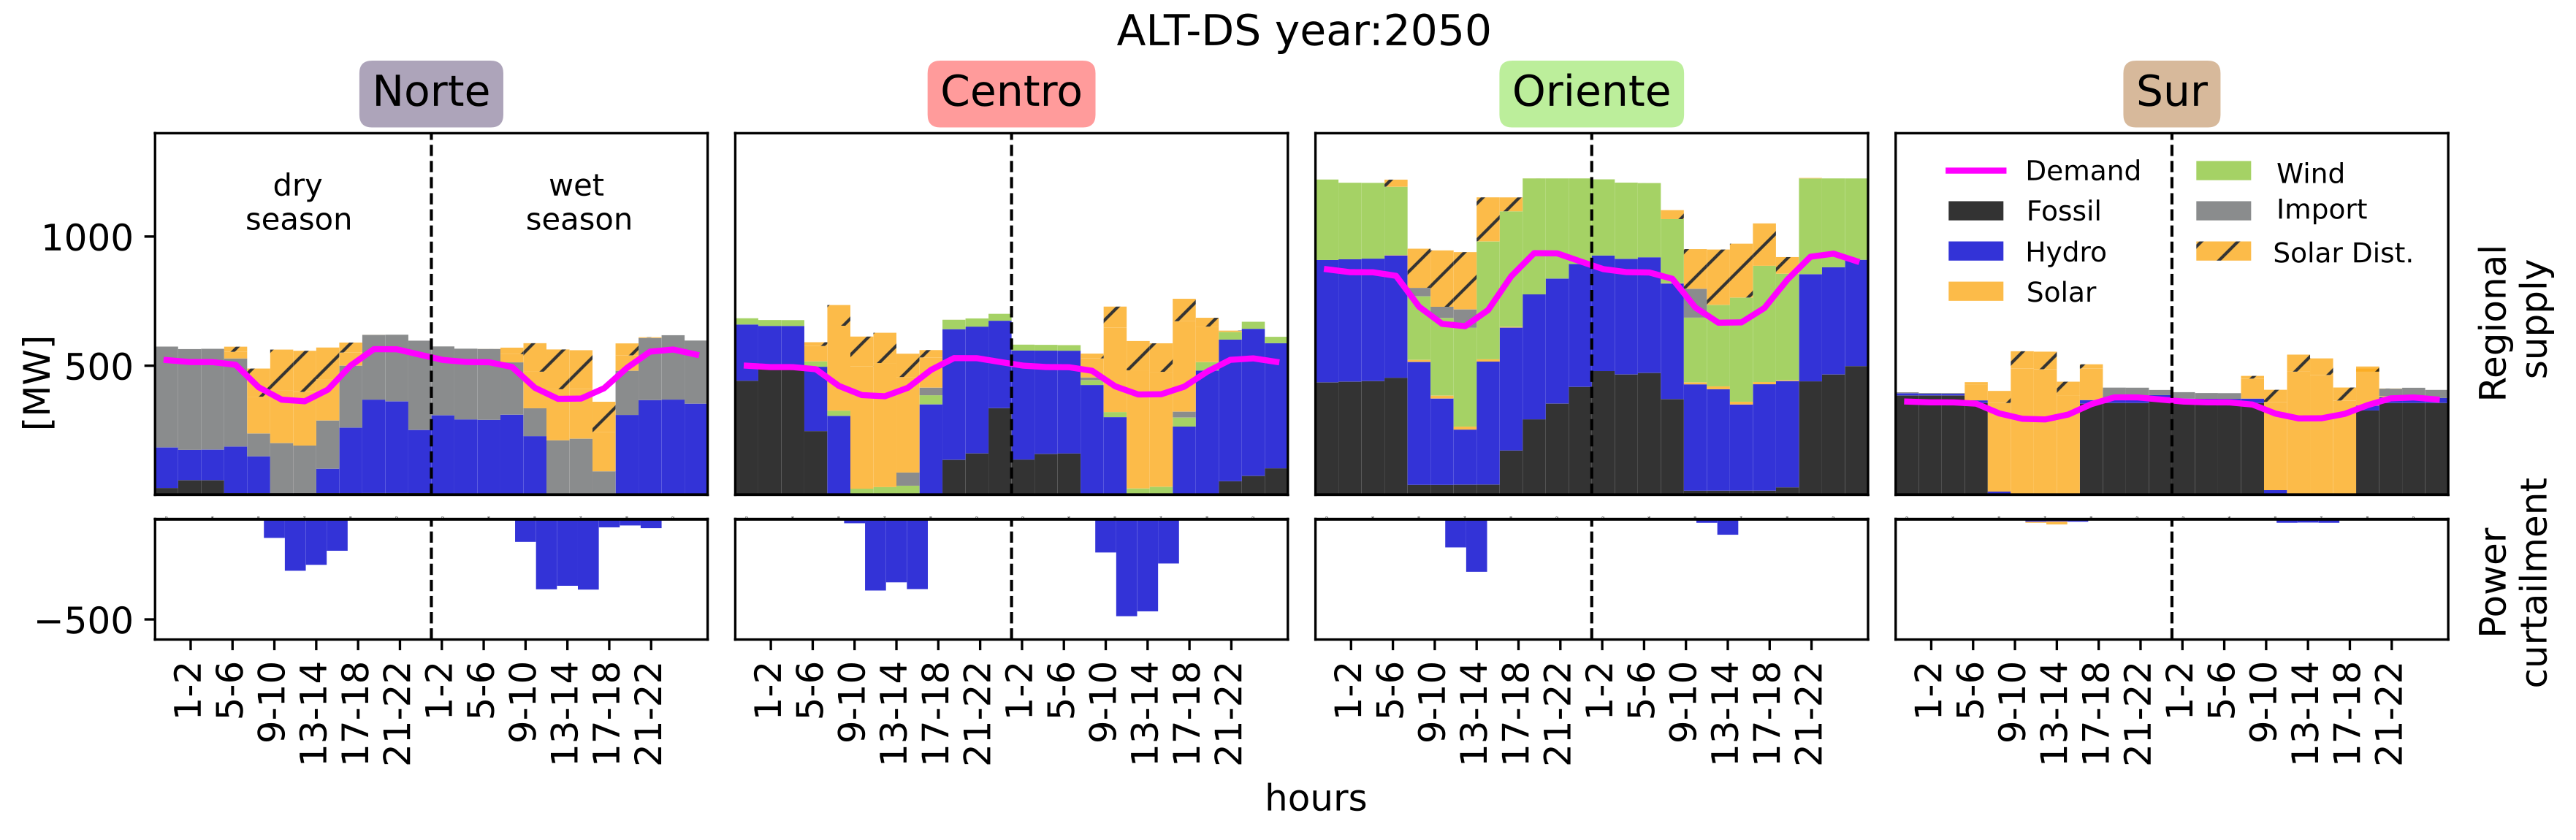
\includegraphics[width=0.9\textwidth, left]{abastALT.png}
	\caption{\label{pow2} Hourly regional power supply (top row) and curtailed power (bottom row) for ALT-DS scenario and year 2050}
\end{figure*}

These preliminary results motivated a more in-depth analysis of the NIS's dispatch and management of future power generation considering that: a large share of the renewable capacity contemplated in the ALT scenario is planned to be installed within a 5-year horizon (Figure \ref{addition}). Current curtailment mitigation strategies include flexibility in power generation, demand-side management, regional complementarity and the use of energy storage in batteries or hydroelectric reservoirs \cite{li2015comprehensive, bird2016wind,berrada2016valuation, denholm2019timescales}, among others. The impact of i) increased flexibility in hydroelectric generation and ii) implementation of battery storage has been evaluated in terms of curtailment reduction.

Hydroelectricity, in particular, provides excellent flexibility services along with low operational costs \cite{liu2023balancing}. In addition, reservoir hydroelectricity can further reduce renewable curtailment by allowing time-shifting generation \cite{denholm2012energy}. Hydroelectricity represents around 50\% of Bolivia's current electricity generation (Table \ref{generation}), and important hydro capacity additions are contemplated in national expansion plans (Figures \ref{addition} and \ref{scenarios}). An alternative daily dispatch scheme for hydroelectricity has been designed for Bolivia's power sector (see Methodology section), and evaluated in terms of impacts in energy curtailment. This implied a thorough analysis of historical hydro generation profiles and stored water levels, and shifting from an existing load-demand oriented operation scheme to a balancing-oriented hydropower operation scheme. In addition to this, we implemented an endogenous battery capacity addition (subject to model optimization).

\begin{figure*}[tp]
	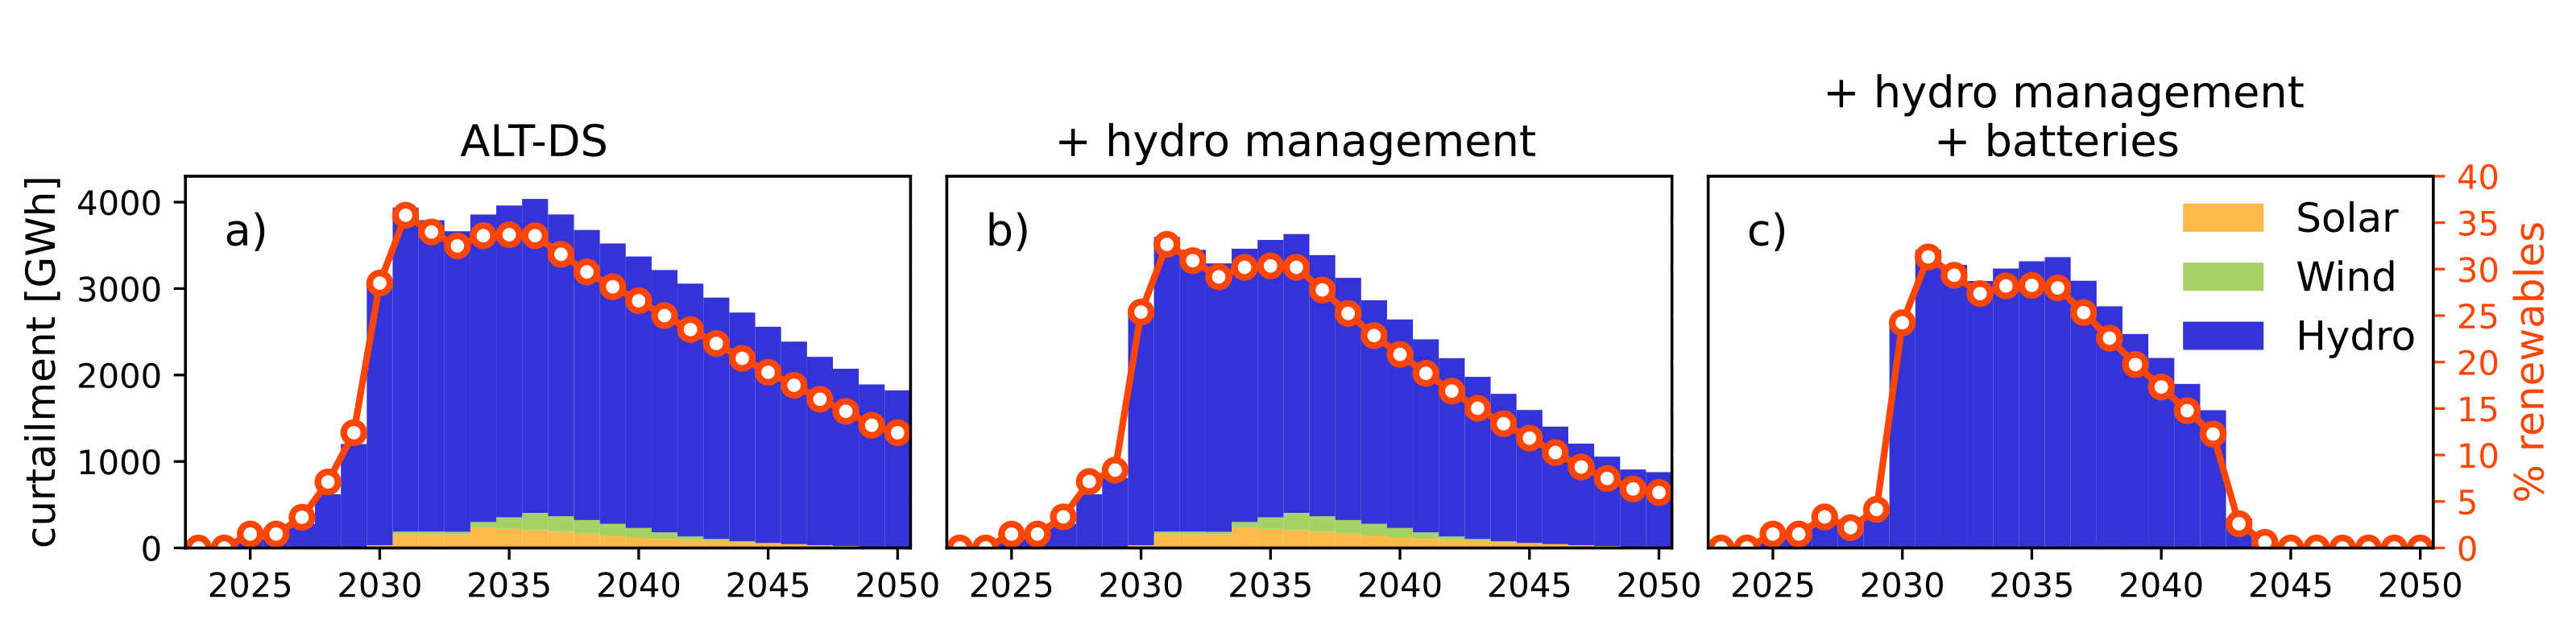
\includegraphics[width=0.9\textwidth, left]{vertimiento.png}
	\caption{\label{vert} Annual curtailed energy for ALT-DS scenario (a), after the implementation of the alternative hydro operation scheme (b) and the endogenous battery capacity addition (c)}
\end{figure*}

The implementation of the alternative hydro management scheme produces a reduction in curtailment that becomes more pronounced toward the end of the simulation period (from 2040 onwards), reducing the percentage of curtailed renewable energy by 50\% relative to the baseline scenario by 2050 (Figure \ref{vert}b)). The addition of battery storage further amplifies this effect, with curtailment declining sharply from 2043 onwards (Figure \ref{vert}c)). Neither strategy, however, proves effective in mitigating the high curtailment rates observed between 2030 and 2040. Looking at capacity and demand projections for this scenario, it becomes evident the temporal mismatch between the early deployment of capacity and the slow-evolving demand (Figure \ref{perc}a)). The magnitude of this oversupply is such that even the average capacity factor of gas-fired power plants remains low (below 10\%) throughout this period, further reducing the margin for thermal displacement and, consequently, the effectiveness of these strategies in mitigating renewable curtailment.

\begin{figure*}[tp]
	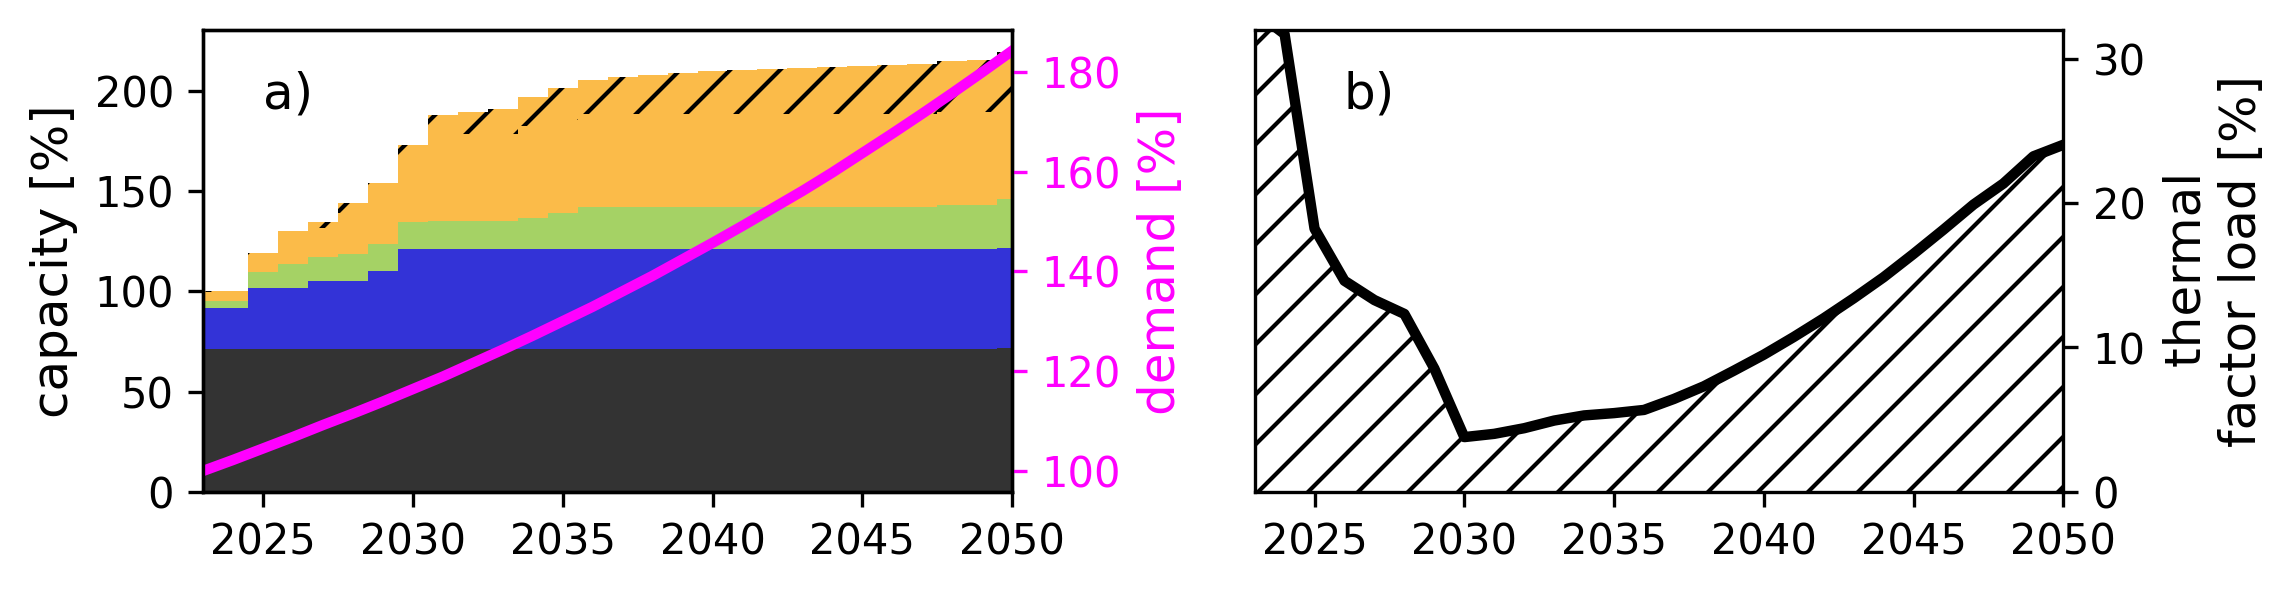
\includegraphics[width=0.8\textwidth, left]{perc.png}
	\caption{\label{perc} Total installed capacity (shadowed areas) and power demand (magenta line) as percentage of the base year (a) and annual load factor of thermal power plants (b) for ALT-DS scenario}
\end{figure*}

\section{Discussion and Conclusions}\label{Conclusions}

This paper presents a modeling exercise of Bolivia's energy system using the LEAP-NEMO model, with a particular focus on renewable penetration scenarios. Results provide valuable insights concerning long-term energy planning and power dispatch schemes. To begin with, the most ambitious scenarios regarding DS capacity show reductions in annual electricity demand of around 9\%. Positive externalities related to the expansion of DS capacity, which include reductions in CO\textsubscript{2}-equivalent emissions and fossil fuel savings, are greater in the BAU-DS scenario - compared with ALT-DS scenario -, in which DS generation displaces thermal generation.

Overall accumulated costs associated with the power system are greater for the ALT scenario (+40\%), which is explained by higher capital costs. The addition of 900 MW of extra DS capacity produces marginal increases in overall costs for both scenarios.

Another novel aspect of this work was the development, for the first time, of a regionalized LEAP-NEMO energy model for Bolivia. This allowed the study of regional power generation and flows within the NIS, and their response to different renewable capacity addition scenarios. Transmission capacities considered in this study do not seem to represent bottlenecks for the evolution of inter-regional power trade throughout the simulation period. Power flows between regions vary according to the evolution of installed capacities within each node. The Centro region stood out as the leading electricity exporter in the BAU scenario. Interannual trend-related growth in electricity demand drives increases in thermal generation in the Centro, Sur and Oriente regions, while generation in the Norte region remains nearly constant throughout the simulation period. Exports are directed towards the Oriente and Sur regions at the beginning of the simulation period, then shift towards the Norte region. In the ALT scenario, the Oriente region becomes an electricity exporter (along with the Centro region) due to considerable renewable capacity additions. Exports are directed towards the Sur region. The addition of extra DS capacity changes regional trade patterns during solar production hours. Moreover, it results in a smaller reduction in thermal generation in the ALT-DS scenario compared with the BAU-DS scenario, while causing a larger reduction in the share of hydro generation in the Centro and Oriente regions.

The results also show that the most ambitious renewable capacity expansion scenario can lead to high levels of curtailment, which the addition of DS capacity further exacerbates. This loss of clean energy limits the displacement of fossil fuel generation and, consequently, the reduction of carbon emissions. Similar behavior has been widely reported in power systems with high renewable shares \cite{li2015comprehensive, o2020too}. In particular, the trajectory described by this scenario resembles the recent experience of Brazil, a historically hydropower-dominated system that has incorporated a substantial share of utility-scale wind and solar as well as distributed solar generation in recent years. As in our results (Figure \ref{pow2}), this rapid expansion has led both to the characteristic midday dip in net load, commonly known as the duck curve, driven by high solar output, and to increasing levels of renewable curtailment during periods of generation surplus \cite{silva2026curtailment}. What is particularly striking about our results, however, is the magnitude of curtailment: in this scenario, renewable curtailment ratios reach 30\%, a value that exceeds most regional \cite{vonpapp2022vertimiento, soto2026wind} and international \cite{cui2020review, yasuda2023latest, vieira2026characterizing} benchmarks.

This variability has motivated research into strategies to mitigate its impacts. Current approaches include flexible generation, demand-side management, grid reinforcement, and energy storage \cite{li2015comprehensive, bird2016wind, berrada2016valuation, denholm2019timescales}. In this study, we explore the most natural of these options for the system under analysis: leveraging its large hydropower capacity to formulate a balancing-oriented dispatch strategy. However, our results show that this strategy alone does not substantially reduce curtailment. We therefore also assess the potential contribution of battery storage. Although a first implementation using realistic capital costs proved economically unfeasible, a scenario neglecting capital costs was evaluated. Even in this case, curtailment ratios were only marginally reduced. Similar outcomes were reported for Greece \cite{psarros2025assessing} and Brazil \cite{da2025regulatory, vieira2025battery}: managing curtailment in power systems with high renewable penetration would require large storage capacities, which would not be economically justifiable. 

The effectiveness of these mitigation strategies is limited by substantial overgeneration, as renewable capacity additions outpace the growth in electricity demand (Figure~\ref{perc}a). This contrasts with the Brazilian case, where curtailment arises mainly from the combination of solar overcapacity and transmission constraints \cite{vieira2026characterizing}. More broadly, conditions of renewable overcapacity and increasing curtailment are far from exceptional: they have been observed in many power systems worldwide \cite{iea2020renewables} and are likely to persist in the near future, driven by continued declines in investment costs \cite{feldman2021us}.

Although this analysis relies on a single demand projection, the results show that a large share of renewable capacity is installed considerably earlier than required by demand growth. Given the magnitude of this mismatch, aligning the pace of centralized and distributed renewable deployment with demand growth appears to be a prerequisite for effective curtailment mitigation. This highlights the importance of integrated planning and policymaking for managing renewable energy deployment. Once this structural overcapacity is addressed, it would be worthwhile to reassess the mitigation strategies implemented in this study, along with others such as demand-side management and regional or international interconnections.

\section{Acknowledgements}

This study was funded by the International Development Research Centre (IDRC), Canada, under grant No. 110091-001 (2023) awarded by the IDRC to Fundación Bariloche.

\clearpage %%Remove this from your manuscript


% Uncomment and use as the case may be
%\begin{theorem} 
%\end{theorem}

% Uncomment and use as the case may be
%\begin{lemma} 
%\end{lemma}

%% The Appendices part is started with the command \appendix;
%% appendix sections are then done as normal sections
%% \appendix

\section{}\label{}

% To print the credit authorship contribution details
\printcredits

%% Loading bibliography style file
%\bibliographystyle{model1-num-names}
\bibliographystyle{cas-model2-names}

% Loading bibliography database
\bibliography{cas-refs}

% Biography
%\bio{}
% Here goes the biography details.
%\endbio

%\bio{pic1}
% Here goes the biography details.
%\endbio

\end{document}

